\chapter{率失真}
\label{chap:rate-distortion}

一个观测站每天只记录“下雨”或“不下雨”，多年统计中下雨的天数约占$30\%$，各天可近似看成相互独立。按第~\ref{chap:lossless-coding}章，若要求每天的记录都被准确还原，长期平均每天至少需要$h_2(0.3)\approx0.881$\,bit，这里$h_2$是以bit计的二元熵。现在放宽要求：允许接收方弄错大约$10\%$的天数。每天还需要多少bit？是直接按$0.881\times0.9$打个折扣，还是能省得更多？

连续取值的信源也有同样的问题。一个标准高斯测量值不可能用有限个bit精确记录，第~\ref{chap:quantization}章用有限个重构值把它装进格子，例如每个值用$1$\,bit的最优两点量化器，均方误差约为$0.363$。这个误差是$1$\,bit能做到的最好结果吗？如果把许多测量值合成一块统一描述，同样每值$1$\,bit，误差最低能降到多少？

这两个问题都在问：给定信源规律和失真标准，平均每个源符号至少需要多少描述。本章先在长块编码中把“可以做到”定义清楚，得到一个由所有方案决定的极限。然后把它与一个只涉及单个符号的优化问题联系起来：在平均失真不超过预算的随机重构规律中，找使互信息最小的一个。这个优化的最小值称为信息率失真函数，率失真编码定理证明它恰好等于长块编码的极限。

有了这个等式，计算就有了两条路。对二元信源与高斯信源，可以先证明一个对所有重构规律成立的信息下界，再构造一个达到它的规律，得到闭式解；开头的两个问题都由此回答。对一般的有限概率表，用Blahut–Arimoto交替算法数值求解。全章以$\operatorname{Bern}(0.3)$信源和Hamming失真为贯穿例子，用标准高斯信源和平方失真评价有限量化器；信息量一律以bit计量。

\section{块重构模型}
\label{sec:rd-block-model}

“至少需要多少描述”要先说清比较的是哪些方案。第~\ref{chap:quantization}章的量化器一次处理一个值，而开头的问题允许把许多天的记录合在一起描述。合在一起之后，一个消息对应一整块重构，失真也要按整块来算。这一节把块编码、码率与失真写成确定的对象，再用块长增长的方案序列定义什么叫“可以做到”。

\paragraph{信源与失真}
设信源依次产生$X_1,X_2,\dots$，它们相互独立，都服从取值空间$\mathcal{X}$上的同一分布$P_X$，这样的信源称为\term{无记忆信源}（memoryless source）。接收方用\term{重构字母表}（reconstruction alphabet）$\hat{\mathcal{X}}$中的值重构，它不必与$\mathcal{X}$相同。与第~\ref{chap:quantization}章一样，重构的好坏由一个失真函数$d:\mathcal{X}\times\hat{\mathcal{X}}\to[0,\infty)$衡量，$d(x,\hat{x})$是把$x$重构成$\hat{x}$的代价。

本章常用两种失真。二元或有限字母表上取$\mathcal{X}=\hat{\mathcal{X}}$，并取
\begin{equation}
  d(x,\hat{x})=\mathbf{1}_{\{x\neq\hat{x}\}},
  \label{eq:rd-hamming}
\end{equation}
它只记对错，称为\term{Hamming失真}（Hamming distortion），平均失真就是重构错误的比例。实值信源取平方失真$d(x,\hat{x})=(x-\hat{x})^{2}$，平均失真就是均方误差。

把$n$个符号合成一块$x^{n}=(x_1,\dots,x_n)$，重构块记为$\hat{x}^{n}$。块的失真取逐符号失真的平均：
\begin{equation}
  d_n(x^{n},\hat{x}^{n})=\frac{1}{n}\sum_{i=1}^{n}d(x_i,\hat{x}_i).
  \label{eq:rd-block-distortion}
\end{equation}
这种按符号相加的失真称为可分失真。取平均而不取总和，是为了让不同块长的方案在“每个符号的失真”上可以直接比较。

\paragraph{块编码}
发送方看到整块$x^{n}$后，只向接收方传一个消息编号；接收方只凭这个编号输出整块重构。图~\ref{fig:rd-block-scheme}画出了这条链路。

\begin{definition}[块编码与码率]
\label{def:rd-block-code}
一个$(n,M)$\term{率失真码}（rate-distortion code）由编码器$f_n:\mathcal{X}^{n}\to\{1,\dots,M\}$与解码器$g_n:\{1,\dots,M\}\to\hat{\mathcal{X}}^{n}$组成。$g_n$的$M$个输出称为码字，它们的集合称为码本。码的码率与期望失真分别是
\begin{equation}
  R=\frac{\log_2M}{n},\qquad
  \mathbb{E}\bigl[d_n\bigl(X^{n},g_n(f_n(X^{n}))\bigr)\bigr],
  \label{eq:rd-rate}
\end{equation}
码率的单位是bit每源符号。
\end{definition}

\begin{BookInlineFigure}
  \centering
  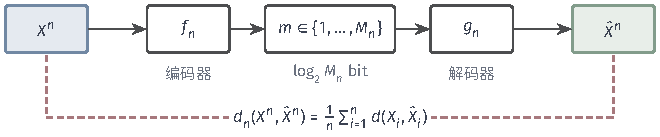
\includegraphics[width=112mm]{figures/07-probability/05-source-coding/tikz/rd-block-scheme/figure.pdf}
  \caption{块重构模型。蓝框是长度为$n$的源块，绿框是重构块。编码器$f_n$把整块映射成$M_n$个编号之一，编号要用约$\log_2M_n$\,bit描述；解码器$g_n$只凭编号输出整块重构。红色虚线表示按式~\eqref{eq:rd-block-distortion}逐符号比较两块。}
  \label{fig:rd-block-scheme}
\end{BookInlineFigure}

$M$不必是$2$的幂。把很多个块连起来发送时，$k$个编号一共有$M^{k}$种组合，用$\lceil k\log_2M\rceil$个bit就能区分，所以$\log_2M$正是每块平均要付出的bit数，除以$n$得到每个源符号的份额。码率只数编号的个数，不涉及编号怎样写成二进制串，也不对编号再作第~\ref{chap:lossless-coding}章的变长压缩；本章所说的码率都是这种固定描述的码率。

码本一旦固定，编码器怎么选最好？对每个$x^{n}$，期望失真中它的那一项是$d_n(x^{n},g_n(f_n(x^{n})))$，只依赖它被送到哪个码字。把每个$x^{n}$送到使$d_n$最小的码字，就同时使每一项最小，期望失真自然最小。所以在给定码本时，最优编码器就是\term{最近码字编码器}（nearest-codeword encoder），一个码本就决定了整个码。这与第~\ref{chap:quantization}章固定重构值后按最近邻划分区域是同一件事，只是“点”换成了整块。

\paragraph{几个简单的码}
回到开头的雨天记录：$X_i\sim\operatorname{Bern}(0.3)$，$1$表示下雨，用Hamming失真。最省的做法是不传任何信息，接收方一律猜“不下雨”。这时$M=1$，码率为$0$，错误比例是下雨的概率：
\[
  R=0,\qquad \mathbb{E}d_n=\mathbb{P}(X_i=1)=0.3 .
\]
另一个极端是逐天照传，$n=1$，$M=2$，码率为$1$，失真为$0$。

块长$n=3$时，可以只用两个码字$\{000,111\}$。在最近码字编码下，一块里$1$的个数$K$不超过$1$时送$000$，否则送$111$，这就是多数表决。$K\sim\operatorname{Bin}(3,0.3)$，
\[
  \begin{gathered}
  \mathbb{P}(K=0)=0.343,\quad \mathbb{P}(K=1)=0.441,\\
  \mathbb{P}(K=2)=0.189,\quad \mathbb{P}(K=3)=0.027 .
  \end{gathered}
\]
$K=1$或$K=2$时恰好错一位，$K=0$或$3$时不错，所以
\[
  \mathbb{E}d_3=\frac{1}{3}\,(0.441+0.189)=0.21,\qquad R=\frac{\log_2 2}{3}=\frac13 .
\]

图~\ref{fig:rd-hamming-cube}把这个码画在三维立方体上。八个顶点是全部源块，相邻顶点只差一位，所以沿棱走一步就是一个Hamming错误。蓝色顶点被送到$000$，黄色顶点被送到$111$，两块区域就是两个码字的最近邻区域。

\begin{BookInlineFigure}
  \centering
  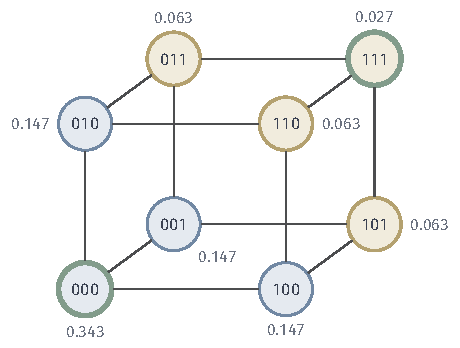
\includegraphics[width=78mm]{figures/07-probability/05-source-coding/tikz/rd-hamming-cube/figure.pdf}
  \caption{块长$3$的码本$\{000,111\}$。立方体的八个顶点是全部源块，旁边的数是它在$\operatorname{Bern}(0.3)$信源下的概率；绿色粗圈是两个码字。蓝色顶点距$000$更近，黄色顶点距$111$更近。蓝色区域的概率是$0.343+3\times0.147=0.784$，其中三个只有一位为$1$的顶点各贡献一个错误。}
  \label{fig:rd-hamming-cube}
\end{BookInlineFigure}

再换一个码本$\{000,100,010,001\}$，$M=4$，码率$\tfrac23$。$K\leq1$的块都能精确重构；$K=2$时最近码字错一位，$K=3$时错两位：
\[
  \mathbb{E}d_3=\frac{1}{3}\,(0.189\times1+0.027\times2)=0.081,\qquad R=\frac{\log_2 4}{3}=\frac23 .
\]
它把码字都放在概率大的地方，利用了“下雨少”这一规律。

还有一种不需要新码本的组合办法。把长块的前一部分符号逐个照传、其余部分一律猜$0$：照传的比例为$\lambda$时，码率为$\lambda$，失真为$0.3(1-\lambda)$。这种在不同方案之间按比例分配符号的做法称为\term{分时}（time sharing），它在码率—失真平面上连出两点之间的线段。

图~\ref{fig:rd-simple-codes}把这些码画在一起。重复码在分时线段的上方：同样码率$\tfrac13$，分时的失真只有$0.2$。四码字的码在线段下方，同样码率$\tfrac23$，分时的失真是$0.1$，它做到了$0.081$。可见简单的组合并不总是最好，块长与码本的选择都影响结果。我们要找的是所有方案都越不过的那条边界。

\begin{BookInlineFigure}
  \centering
  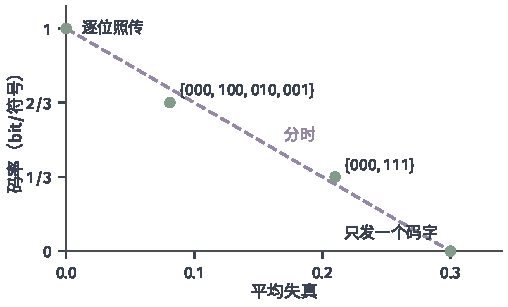
\includegraphics[width=86mm]{figures/07-probability/05-source-coding/matplotlib/rd-simple-codes/figure.pdf}
  \caption{$\operatorname{Bern}(0.3)$信源在Hamming失真下几个简单码的码率与平均失真（绿点）：只发一个码字、逐位照传、块长$3$的重复码$\{000,111\}$和码本$\{000,100,010,001\}$。紫色虚线是前两个方案之间的分时。}
  \label{fig:rd-simple-codes}
\end{BookInlineFigure}

\paragraph{渐近可达性}
单个块长的码受到整数效应的牵制：$M$只能是整数，码字只能放在格点上。为了得到一个干净的极限，我们看块长不断增长的一列码。

\begin{definition}[可达码率失真对]
\label{def:rd-achievable}
若对每个$n\geq1$都有一个$(n,M_n)$码，使
\begin{equation}
  \limsup_{n\to\infty}\frac{\log_2M_n}{n}\leq R,\qquad
  \limsup_{n\to\infty}\mathbb{E}\bigl[d_n\bigl(X^{n},g_n(f_n(X^{n}))\bigr)\bigr]\leq D,
  \label{eq:rd-achievable}
\end{equation}
则称$(R,D)$为\term{可达码率失真对}（achievable rate-distortion pair）。对给定的$D$，所有使$(R,D)$可达的$R$的下确界记为$R_{\mathrm{op}}(D)$，称为\term{操作率失真函数}（operational rate-distortion function）。
\end{definition}

定义中两个上极限分别留出了余地：码率可以比$R$稍大，只要最终不超过$R$；失真也一样。有限块长的码不在定义之内，它们只是这一列中的成员。若$(R,D)$可达，那么任何更大的$R'$与$D'$也可达，所以可达的点组成码率—失真平面中一块向右上方延伸的区域，$R_{\mathrm{op}}$是它的下边界。

\paragraph{三种失真要求}
“失真不超过$D$”还可以有别的读法，它们给出不同的极限，需要事先分清。式~\eqref{eq:rd-achievable}用的是期望失真：对源块的分布平均以后不超过$D$，个别块的失真可以很大。第二种是逐块保证，要求每一个可能的源块都满足$d_n\leq D$。第三种是超额失真概率要求，即
\[
  \mathbb{P}\bigl(d_n(X^{n},\hat{X}^{n})>D\bigr)\to0 ,
\]
允许失真超标，但超标的概率要趋于零。

若失真有上界$d_{\max}=\max_{x,\hat{x}}d(x,\hat{x})<\infty$，后两种要求都强于期望失真要求。把期望按是否超标分成两部分：
\[
  \mathbb{E}d_n\leq D\cdot\mathbb{P}(d_n\leq D)+d_{\max}\,\mathbb{P}(d_n>D)
  \leq D+d_{\max}\,\mathbb{P}(d_n>D).
\]
超额失真概率趋零时右端趋于$D$，所以满足第三种要求的码列也满足期望失真要求。反过来不成立：对一半的块照传、另一半一律猜$0$的码，期望失真可以很小，超标概率却始终是$\tfrac12$。

逐块保证则可能贵得多。仍看Hamming失真与$0<D<\tfrac12$。一个码字能“照顾”到的源块，是与它相差不超过$nD$位的那些，个数至多为$\sum_{k\leq nD}\binom{n}{k}$。对$t=D/(1-D)\leq1$，二项展开给出
\[
  1=\sum_{k=0}^{n}\binom{n}{k}D^{k}(1-D)^{n-k}
  \geq\sum_{k\leq nD}\binom{n}{k}(1-D)^{n}t^{k}
  \geq\sum_{k\leq nD}\binom{n}{k}(1-D)^{n}t^{nD},
\]
这里第二个不等号用了$k\leq nD$与$t\leq1$。而$(1-D)^{n}t^{nD}=D^{nD}(1-D)^{n-nD}=2^{-nh_2(D)}$，其中$h_2(t)=-t\log_2t-(1-t)\log_2(1-t)$是二元熵。于是
\[
  \sum_{k\leq nD}\binom{n}{k}\leq2^{nh_2(D)} .
\]

要照顾到全部$2^{n}$个源块，码字个数必须满足$M_n\cdot2^{nh_2(D)}\geq2^{n}$，即
\[
  \frac{\log_2M_n}{n}\geq1-h_2(D).
\]
这个界与下雨的概率$0.3$完全无关：概率再小的块也必须被照顾。取$D=0.1$，右端为$1-h_2(0.1)\approx0.531$\,bit。第~\ref{sec:rd-binary}节将算出期望失真标准下只需约$0.412$\,bit，差别就来自是否允许罕见的块失真偏大。

逐块保证适合要防最坏情况的场合，超额失真概率适合要控制“几乎每块”的场合。本章以期望失真为共同标准，它与平均码长一样关心长期平均表现，也是第~\ref{chap:quantization}章评价量化器的标准。


\section{信息率失真函数}
\label{sec:rd-information-rd}

$R_{\mathrm{op}}(D)$的定义涉及所有块长、所有码本，无法直接计算。我们需要一个只看单个符号就能算的量，并且它要与码的描述能力挂钩。互信息正好起这个作用。

设$(n,M)$码的重构块为$\hat{X}^{n}=g_n(f_n(X^{n}))$。它由编号决定，至多取$M$个值，所以它能携带的关于$X^{n}$的信息有限：
\[
  I(X^{n};\hat{X}^{n})\leq H(\hat{X}^{n})\leq\log_2M=nR .
\]
第一个不等号来自
\[
  I(X^{n};\hat{X}^{n})=H(\hat{X}^{n})-H(\hat{X}^{n}\mid X^{n})
\]
与条件熵非负，第二个是取$M$个值的变量熵不超过$\log_2M$。所以码率至少要容纳重构与源之间的互信息。重构必须足够接近源，这又迫使互信息不能太小。下面在单个符号上精确地表述这种张力：失真不超过$D$时，互信息最少是多少。

这里沿用第~\ref{chap:information-measures}章的熵、条件熵与互信息，只把对数换成以$2$为底，数值都除以$\ln2$，单位从nat变成bit。有限字母表上，
\[
  I(X;\hat{X})=\sum_{x,\hat{x}}p(x,\hat{x})\log_2\frac{p(x,\hat{x})}{p(x)\,r(\hat{x})},
\]
其中$r$是$\hat{X}$的分布；它就是联合分布相对边缘乘积的KL散度，非负，且为零当且仅当$X$与$\hat{X}$独立。

\subsection{重构条件分布}
\label{sec:rd-test-channels}

单个符号上，一个“重构规律”就是给定源值$x$时，重构值怎样选择。允许这种选择带有随机性，用条件分布描述它。

设$\mathcal{X}$与$\hat{\mathcal{X}}$是有限集，$p(x)=P_X(\{x\})$。一个\term{测试信道}（test channel）是一族条件概率$q(\hat{x}\mid x)\geq0$，对每个$x$有$\sum_{\hat{x}}q(\hat{x}\mid x)=1$。它与源分布一起确定联合分布$p(x)q(\hat{x}\mid x)$，重构的边缘分布是
\begin{equation}
  r_q(\hat{x})=\sum_{x}p(x)\,q(\hat{x}\mid x).
  \label{eq:rd-output-marginal}
\end{equation}
把$q$看作一个随机的“重构器”：输入$x$，按$q(\cdot\mid x)$抽一个$\hat{x}$输出。它的平均失真与互信息分别是
\begin{equation}
  \mathbb{E}d(X,\hat{X})=\sum_{x,\hat{x}}p(x)\,q(\hat{x}\mid x)\,d(x,\hat{x}),
  \label{eq:rd-test-distortion}
\end{equation}
\begin{equation}
  I(P_X,q)=\sum_{x,\hat{x}}p(x)\,q(\hat{x}\mid x)\log_2\frac{q(\hat{x}\mid x)}{r_q(\hat{x})}.
  \label{eq:rd-test-information}
\end{equation}
式~\eqref{eq:rd-test-information}中约定$0\log_20=0$；若$p(x)q(\hat{x}\mid x)>0$，则$r_q(\hat{x})>0$，分母不会为零。

\begin{definition}[信息率失真函数]
\label{def:rd-information-rd}
给定源分布$P_X$与失真函数$d$，对$D\geq0$令
\begin{equation}
  R(D)=\inf\Bigl\{I(P_X,q):\ q\text{为测试信道},\ \mathbb{E}d(X,\hat{X})\leq D\Bigr\},
  \label{eq:rd-information-rd}
\end{equation}
约定空集的下确界为$+\infty$。$R(D)$称为\term{信息率失真函数}（information rate-distortion function），单位是bit每源符号。
\end{definition}

式~\eqref{eq:rd-information-rd}的优化变量只有测试信道$q$。源分布$P_X$是给定的，不参与优化；改变的只是“看到$x$以后怎样重构”。下一部分研究信道时问题方向相反：信道的条件分布固定，改变的是输入分布。两个问题都优化互信息，但一个求最小、一个求最大，变量也不同。

测试信道是一个理论对象，不是编码器。真正的编码器看到整块源符号，确定地输出一个编号；测试信道只作用在单个符号上，并且允许抛硬币。它在本章有两个用处：在第~\ref{sec:rd-coding-theorem}节的下界证明中，任意块编码都会诱导出一个测试信道；在可达性证明中，最优测试信道指导怎样随机生成码本。$R(D)$与$R_{\mathrm{op}}(D)$相等是需要证明的定理，现在只把$R(D)$当作一个优化问题来研究。

一般的取值空间中，测试信道是从$\mathcal{X}$到$\hat{\mathcal{X}}$的Markov核（第~\ref{chap:conditional-distributions}章），互信息用联合分布相对边缘乘积的KL散度定义，允许取$+\infty$，式~\eqref{eq:rd-information-rd}的写法不变。本节余下部分先在有限字母表上讨论，一般情形放在第~\ref{sec:rd-feasible-range}节末尾。

\paragraph{三个测试信道}
仍取$X\sim\operatorname{Bern}(0.3)$与Hamming失真。第一个测试信道不看输入，一律输出$0$。这时$\hat{X}$是常数，与$X$独立，
\[
  I=0,\qquad \mathbb{E}d=\mathbb{P}(X=1)=0.3 .
\]

第二个测试信道以概率$0.1$把输入翻转：$q(1\mid0)=q(0\mid1)=0.1$。平均失真正好是翻转概率$0.1$。由式~\eqref{eq:rd-output-marginal}，
\[
  r_q(1)=0.7\times0.1+0.3\times0.9=0.34 .
\]
给定$X$时$\hat{X}$的熵是$h_2(0.1)$，于是
\[
  I=H(\hat{X})-H(\hat{X}\mid X)=h_2(0.34)-h_2(0.1)\approx0.9248-0.4690=0.4558 .
\]

第三个测试信道取$q(1\mid0)=\tfrac1{28}$，$q(0\mid1)=\tfrac14$：常见的$0$几乎不动，罕见的$1$有四分之一被改成$0$。平均失真仍然是
\[
  \mathbb{E}d=0.7\times\frac{1}{28}+0.3\times\frac14=0.025+0.075=0.1 .
\]
重构边缘为
\[
  r_q(1)=0.7\times\frac1{28}+0.3\times\frac34=0.25 .
\]

给定$X=0$与$X=1$时$\hat{X}$的熵分别是$h_2(\tfrac1{28})$与$h_2(\tfrac14)$，按$p(x)$平均得条件熵，于是
\[
  I=h_2(0.25)-0.7\,h_2\Bigl(\frac1{28}\Bigr)-0.3\,h_2\Bigl(\frac14\Bigr)
  \approx0.8113-0.1556-0.2434=0.4123 .
\]
同样的失真，第三个信道比第二个少用了约$0.044$\,bit的信息。它把错误集中在罕见符号上：把一个$1$改成$0$让重构更“像”最常见的结果，重构本身更可预测，需要的描述更少。第~\ref{sec:rd-binary}节将证明$0.4123$正是$R(0.1)$。

图~\ref{fig:rd-test-channel-cloud}把所有二元测试信道一次画出来。$q(1\mid0)$与$q(0\mid1)$各取网格上的值，每个测试信道对应一个点（平均失真，互信息）。$R(D)$就是这团点云的下边界：在竖线$D$的左侧所有点中，最低的高度。

\begin{BookInlineFigure}
  \centering
  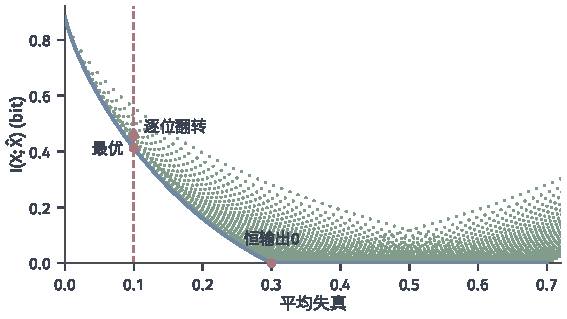
\includegraphics[width=96mm]{figures/07-probability/05-source-coding/matplotlib/rd-test-channel-cloud/figure.pdf}
  \caption{$\operatorname{Bern}(0.3)$信源与Hamming失真下全部二元测试信道的平均失真与互信息。绿点：$q(1\mid0)$与$q(0\mid1)$各取$0,\tfrac1{60},\dots,1$共$61\times61$个组合。蓝线是点云的下边界$R(D)$，其公式在第~\ref{sec:rd-binary}节导出。红点依次是以$0.1$翻转的测试信道、$D=0.1$时的最优测试信道和恒输出$0$；红色虚线是$D=0.1$。}
  \label{fig:rd-test-channel-cloud}
\end{BookInlineFigure}

\subsection{单调性与凸性}
\label{sec:rd-convexity}

点云的下边界看上去单调下降、向下凸。单调性只需比较可行集合。

失真预算放宽时，满足$\mathbb{E}d\leq D$的测试信道都满足$\mathbb{E}d\leq D'$，其中$D<D'$。在更大的集合上取下确界只会更小，所以$R(D')\leq R(D)$，$R$非增。

凸性来自互信息对测试信道的凸性。证明要用一个关于两组非负数的不等式，它把KL散度非负的论证推广到未归一化的数组。

\begin{lemma}[对数和不等式]
\label{lem:rd-log-sum}
设$a_1,\dots,a_k\geq0$，$b_1,\dots,b_k>0$，$a=\sum_ia_i$，$b=\sum_ib_i$。则
\begin{equation}
  \sum_{i=1}^{k}a_i\log_2\frac{a_i}{b_i}\geq a\log_2\frac{a}{b},
  \label{eq:rd-log-sum}
\end{equation}
约定$0\log_20=0$。
\end{lemma}

\begin{proof}
$a=0$时两边都为$0$。设$a>0$，记$\phi(t)=t\log_2t$（$\phi(0)=0$），它在$[0,\infty)$上凸，因为$t>0$时$\phi''(t)=1/(t\ln2)>0$。左端可以写成
\[
  \sum_{i}a_i\log_2\frac{a_i}{b_i}=b\sum_{i}\frac{b_i}{b}\,\phi\Bigl(\frac{a_i}{b_i}\Bigr).
\]
权重$b_i/b$非负且和为$1$，由Jensen不等式，
\[
  \sum_{i}\frac{b_i}{b}\,\phi\Bigl(\frac{a_i}{b_i}\Bigr)\geq\phi\Bigl(\sum_{i}\frac{b_i}{b}\cdot\frac{a_i}{b_i}\Bigr)=\phi\Bigl(\frac{a}{b}\Bigr)=\frac{a}{b}\log_2\frac{a}{b}.
\]
两边乘以$b$即得式~\eqref{eq:rd-log-sum}。
\end{proof}

\begin{lemma}[互信息对测试信道的凸性]
\label{lem:rd-mi-convex}
固定有限字母表上的源分布$P_X$。对测试信道$q_1,q_2$与$\lambda\in[0,1]$，令$q_\lambda=\lambda q_1+(1-\lambda)q_2$，则
\begin{equation}
  I(P_X,q_\lambda)\leq\lambda\,I(P_X,q_1)+(1-\lambda)\,I(P_X,q_2).
  \label{eq:rd-mi-convex}
\end{equation}
\end{lemma}

\begin{proof}
$q_\lambda$的每一行仍是概率分布，所以它是测试信道。固定一对$(x,\hat{x})$，记
\[
  a_j=p(x)\,q_j(\hat{x}\mid x),\qquad b_j=p(x)\,r_{q_j}(\hat{x}),\qquad j=1,2 .
\]
由式~\eqref{eq:rd-output-marginal}，$r_q$对$q$是线性的，所以$q_\lambda$对应的两个量正好是$\lambda a_1+(1-\lambda)a_2$与$\lambda b_1+(1-\lambda)b_2$。

式~\eqref{eq:rd-test-information}在$(x,\hat{x})$处的项是$a\log_2(a/b)$的形式。对两项$\lambda a_1,(1-\lambda)a_2$与$\lambda b_1,(1-\lambda)b_2$用引理~\ref{lem:rd-log-sum}（分母为零的项分子也为零，可以略去），得
\[
  \bigl(\lambda a_1+(1-\lambda)a_2\bigr)\log_2\frac{\lambda a_1+(1-\lambda)a_2}{\lambda b_1+(1-\lambda)b_2}
  \leq\lambda\,a_1\log_2\frac{a_1}{b_1}+(1-\lambda)\,a_2\log_2\frac{a_2}{b_2}.
\]
对所有$(x,\hat{x})$求和，左端是$I(P_X,q_\lambda)$，右端是式~\eqref{eq:rd-mi-convex}的右端。
\end{proof}

\begin{theorem}[$R(D)$的单调性与凸性]
\label{thm:rd-convex}
有限字母表上，$R$在$[0,\infty)$上非增。在$R$取有限值的区间上，对任意$D_1,D_2$与$\lambda\in[0,1]$，
\begin{equation}
  R\bigl(\lambda D_1+(1-\lambda)D_2\bigr)\leq\lambda R(D_1)+(1-\lambda)R(D_2).
  \label{eq:rd-convex}
\end{equation}
\end{theorem}

\begin{proof}
非增性已经说明。取$\varepsilon>0$，按下确界的定义取测试信道$q_1,q_2$，使
\[
  \mathbb{E}_{q_j}d\leq D_j,\qquad I(P_X,q_j)\leq R(D_j)+\varepsilon,\qquad j=1,2 .
\]
式~\eqref{eq:rd-test-distortion}对$q$是线性的，所以$q_\lambda$的平均失真是
\[
  \lambda\,\mathbb{E}_{q_1}d+(1-\lambda)\,\mathbb{E}_{q_2}d\leq\lambda D_1+(1-\lambda)D_2 ,
\]
$q_\lambda$在后者的可行集合中。

由$R$的定义与引理~\ref{lem:rd-mi-convex}，
\[
  R\bigl(\lambda D_1+(1-\lambda)D_2\bigr)\leq I(P_X,q_\lambda)
  \leq\lambda R(D_1)+(1-\lambda)R(D_2)+\varepsilon .
\]
令$\varepsilon\to0$即得式~\eqref{eq:rd-convex}。
\end{proof}

证明中把两个测试信道按比例混合：对每个输入，先以概率$\lambda$决定用$q_1$还是$q_2$，再按选中的那个重构。失真随混合线性变化，互信息却至多线性变化，这就是凸性。

块编码中的分时是同一想法的操作版本。设两列码分别达到$(R_1,D_1)$与$(R_2,D_2)$。块长为$n$时，前$\lfloor\lambda n\rfloor$个符号用第一列中相应块长的码，其余符号用第二列的码，编号合起来发送。码率与失真都按符号比例加权，趋于$\lambda R_1+(1-\lambda)R_2$与$\lambda D_1+(1-\lambda)D_2$，所以可达区域也是凸的。

图~\ref{fig:rd-convexity}比较这两种混合。$q_1$是照传，$q_2$是恒输出$0$，各取一半。混合后的测试信道在$X=0$时输出$0$，在$X=1$时以$\tfrac12$的概率输出$1$，失真为$0.15$。由$r_q(1)=0.15$与$H(\hat{X}\mid X)=0.3\,h_2(\tfrac12)$，它的互信息是
\[
  I=h_2(0.15)-0.3\approx0.6098-0.3=0.3098 .
\]
这低于两端点连线在$D=0.15$处的高度$0.4406$。同样比例的分时只能落在连线上，混合测试信道已经越过了它；而$R(0.15)\approx0.2715$又比混合更低。

\begin{BookInlineFigure}
  \centering
  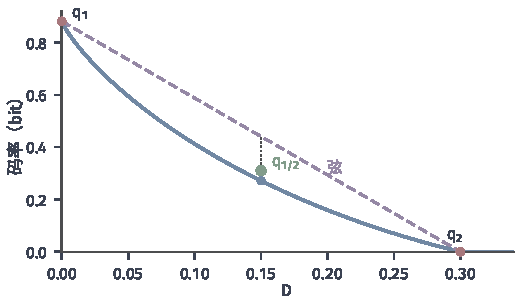
\includegraphics[width=88mm]{figures/07-probability/05-source-coding/matplotlib/rd-convexity/figure.pdf}
  \caption{$\operatorname{Bern}(0.3)$与Hamming失真下$R(D)$的凸性。红点$q_1$是照传（$D=0$，$I=h_2(0.3)$），$q_2$是恒输出$0$（$D=0.3$，$I=0$），紫色虚线是两者之间的弦，也是分时所能达到的点。绿点是两个测试信道各占一半的混合，高$0.3098$，蓝点是同一失真$0.15$下的$R(0.15)\approx0.2715$。}
  \label{fig:rd-convexity}
\end{BookInlineFigure}

\subsection{可行范围与零码率失真}
\label{sec:rd-feasible-range}

$R(D)$在哪些$D$上有限，在哪里降到零？下确界能否取到？这些问题决定了曲线的两个端点，也为编码定理的证明提供需要的连续性。本小节先设$\mathcal{X}$与$\hat{\mathcal{X}}$有限，$d$取非负有限值。

\paragraph{最小可行失真}
任何测试信道的平均失真都不会低于“每个源值都用它最好的重构”时的失真。对每个$x$，$d(x,\cdot)$按$q(\cdot\mid x)$的平均不小于它的最小值，再按$p(x)$平均得到$\mathbb{E}d\geq D_{\min}$，其中
\begin{equation}
  D_{\min}=\sum_{x}p(x)\min_{\hat{x}}d(x,\hat{x}).
  \label{eq:rd-dmin}
\end{equation}
把每个$x$确定地送到一个使$d(x,\cdot)$最小的$\hat{x}$，就达到$D_{\min}$。所以$D<D_{\min}$时可行集合为空，$R(D)=+\infty$；$D\geq D_{\min}$时可行集合非空。

另一端，若$\hat{X}$与$X$独立，平均失真是对重构边缘$r$的加权平均：
\[
  \mathbb{E}d=\sum_{\hat{x}}r(\hat{x})\sum_{x}p(x)d(x,\hat{x})\geq\min_{\hat{x}}\sum_{x}p(x)d(x,\hat{x}).
\]
右端记为
\begin{equation}
  D_{\max}=\min_{\hat{x}\in\hat{\mathcal{X}}}\sum_{x}p(x)\,d(x,\hat{x}),
  \label{eq:rd-dmax}
\end{equation}
它是只输出一个最佳常量时的失真，称为\term{零码率失真}（zero-rate distortion）。只输出一个常量不需要任何描述，所以$D\geq D_{\max}$时$R(D)=0$。

\begin{theorem}[最优测试信道的存在与$R$的连续性]
\label{thm:rd-existence}
设$\mathcal{X},\hat{\mathcal{X}}$有限，$d$非负有限。对每个$D\geq D_{\min}$，式~\eqref{eq:rd-information-rd}中的下确界可以取到，并且$R(D)\leq H(X)$。$R$在$[D_{\min},\infty)$上连续。
\end{theorem}

\begin{proof}
把测试信道看成$\mathbb{R}^{\lvert\mathcal{X}\rvert\times\lvert\hat{\mathcal{X}}\rvert}$中的矩阵。各行非负且和为$1$的矩阵组成有界闭集，式~\eqref{eq:rd-test-distortion}对$q$线性，$\mathbb{E}d\leq D$是一个闭的半空间。两者之交$\mathcal{Q}(D)$是非空紧集。

互信息对$q$连续。把式~\eqref{eq:rd-test-information}中的对数拆开，并按式~\eqref{eq:rd-output-marginal}合并$\hat{x}$相同的项，得
\[
  I(P_X,q)=\sum_{x,\hat{x}}p(x)\,\phi\bigl(q(\hat{x}\mid x)\bigr)-\sum_{\hat{x}}\phi\bigl(r_q(\hat{x})\bigr),
\]
其中$\phi(t)=t\log_2t$在$[0,1]$上连续，$r_q$对$q$线性。连续函数在非空紧集上取到最小值，所以下确界可以取到。又$I(P_X,q)\leq H(X)$对一切$q$成立，因为$I=H(X)-H(X\mid\hat{X})$，故$R(D)\leq H(X)$。

连续性先看内部。$R$在$[D_{\min},\infty)$上取有限值并且是凸函数，开区间上的凸函数连续，所以$R$在$(D_{\min},\infty)$上连续。

在端点$D_{\min}$处，取$D_k\downarrow D_{\min}$与相应的最优测试信道$q_k\in\mathcal{Q}(D_k)$。所有$q_k$落在紧集$\mathcal{Q}(D_1)$中，取收敛子列$q_{k_j}\to q$。由失真的线性与连续性，$q$的平均失真不超过$D_{\min}$，于是
\[
  R(D_{\min})\leq I(P_X,q)=\lim_{j\to\infty}R(D_{k_j}).
\]
另一方面$R$非增，$R(D_{k_j})\leq R(D_{\min})$。两边夹住，$R(D_k)\to R(D_{\min})$。
\end{proof}

\begin{theorem}[零码率失真]
\label{thm:rd-zero-rate}
在定理~\ref{thm:rd-existence}的条件下，$R(D)=0$当且仅当$D\geq D_{\max}$。在$[D_{\min},D_{\max}]$上$R$严格递减。
\end{theorem}

\begin{proof}
$D\geq D_{\max}$时恒输出最佳常量可行，互信息为零。反之设$R(D)=0$，由定理~\ref{thm:rd-existence}，存在可行的$q$使$I(P_X,q)=0$，即$X$与$\hat{X}$独立。由式~\eqref{eq:rd-dmax}前的计算，它的平均失真至少为$D_{\max}$，所以$D\geq D_{\max}$。

严格递减用反证。设$D_{\min}\leq D_1<D_2\leq D_{\max}$且$R(D_1)=R(D_2)$。由刚证明的结论，$D_1<D_{\max}$蕴含$R(D_1)>0$。若$D_2<D_{\max}$，把$D_2$写成$D_1$与$D_{\max}$的凸组合$D_2=\lambda D_1+(1-\lambda)D_{\max}$，$\lambda\in(0,1)$，由式~\eqref{eq:rd-convex}，
\[
  R(D_2)\leq\lambda R(D_1)+(1-\lambda)\cdot0<R(D_1),
\]
其中最后一步用了$R(D_1)>0$，与假设矛盾。若$D_2=D_{\max}$，则$R(D_1)=0$，与$D_1<D_{\max}$矛盾。
\end{proof}

当$\mathcal{X}=\hat{\mathcal{X}}$且$d(x,\hat{x})=0$当且仅当$x=\hat{x}$时，$D_{\min}=0$，而$\mathbb{E}d=0$迫使$\hat{X}=X$，于是$R(0)=I(X;X)=H(X)$。零失真的码率回到第~\ref{chap:lossless-coding}章的熵。雨天记录的例子中$D_{\min}=0$，$R(0)=h_2(0.3)$；零码率失真$D_{\max}=\min\{0.3,0.7\}=0.3$，就是一律猜“不下雨”。

\paragraph{一个$D_{\min}>0$的例子}
设$X$在$\{0,1,2\}$上取值，概率为$(0.3,0.4,0.3)$，而重构只能取$\hat{\mathcal{X}}=\{0,2\}$，失真为平方误差。$x=1$离两个重构值都是$1$，所以由式~\eqref{eq:rd-dmin}，
\[
  D_{\min}=0.4\times1=0.4 .
\]
两个常量重构的平均失真都是$0.4\times1+0.3\times4=1.6$，所以$D_{\max}=1.6$。

$D=D_{\min}$时，$0$必须重构为$0$，$2$必须重构为$2$，否则会多出$4$的失真；只有$x=1$可以自由选择。设它以概率$a$重构为$2$，则$\mathbb{P}(\hat{X}=2)=0.3+0.4a$，$H(\hat{X}\mid X)=0.4\,h_2(a)$，
\[
  I(a)=h_2(0.3+0.4a)-0.4\,h_2(a).
\]

用$h_2'(t)=\log_2\frac{1-t}{t}$求导，
\[
  I'(a)=0.4\log_2\frac{0.7-0.4a}{0.3+0.4a}-0.4\log_2\frac{1-a}{a}.
\]
令其为零，得$a(0.7-0.4a)=(1-a)(0.3+0.4a)$，展开后$0.7a=0.3+0.1a$，即$a=\tfrac12$。$I$是测试信道的凸函数，在这条线段上也凸，所以这是最小点：
\[
  R(D_{\min})=I\Bigl(\frac12\Bigr)=h_2(0.5)-0.4=0.6 .
\]
对照$a=0$时的$h_2(0.3)\approx0.881$与源熵$H(X)\approx1.571$：零失真不可行，在最小失真处也不必把源描述得一清二楚，那个处在中间、怎样重构都一样差的符号正好用来“抛硬币”。

图~\ref{fig:rd-ternary-range}画出这个例子的整条曲线。左侧浅红区域不可行；曲线从$(0.4,0.6)$开始，严格下降，在$D_{\max}=1.6$处降到零，之后保持为零。

\begin{BookInlineFigure}
  \centering
  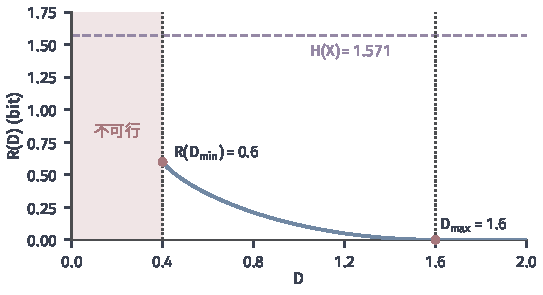
\includegraphics[width=92mm]{figures/07-probability/05-source-coding/matplotlib/rd-ternary-range/figure.pdf}
  \caption{三元信源$p=(0.3,0.4,0.3)$、重构字母表$\{0,2\}$与平方失真的$R(D)$（蓝线），由第~\ref{sec:rd-computation}节的算法逐点计算。浅红区域$D<D_{\min}=0.4$不可行；红点是$(D_{\min},0.6)$与$(D_{\max},0)$；紫色虚线是源熵$H(X)\approx1.571$\,bit。}
  \label{fig:rd-ternary-range}
\end{BookInlineFigure}

\paragraph{一般重构空间}
重构值取实数或其他无限集合时，上面每一步都要重新核对。$d$需要对乘积$\sigma$代数可测，平均失真才有定义；可行的Markov核要组成某种意义下的紧集，互信息要对这种收敛下半连续，下确界才能取到。这些条件并不自动成立。

设$X\sim\operatorname{Bern}(\tfrac12)$，重构只能取开区间$(0,1)$中的值，$d(x,\hat{x})=\lvert x-\hat{x}\rvert$。把式~\eqref{eq:rd-dmin}中的最小值换成下确界，$D_{\min}$仍是$0$，但没有重构值能让失真为零，平均失真为$0$的测试信道不存在，$R(0)=+\infty$。

另一方面，对任意$\varepsilon\in(0,\tfrac12)$，把$0$重构为$\varepsilon$、把$1$重构为$1-\varepsilon$，平均失真为$\varepsilon$，互信息为$1$。所以$R(D)\leq1$对一切$D>0$成立，$R$在$0$处从有限值跳到$+\infty$。这里$\hat{\mathcal{X}}$不紧，下确界“存在”只是一个数，最优重构并未取到，定理~\ref{thm:rd-existence}的结论也随之失效。


\section{率失真编码定理}
\label{sec:rd-coding-theorem}

现在有两个函数：$R_{\mathrm{op}}(D)$由所有块编码决定，$R(D)$由单个符号上的优化决定。本节证明它们相等。证明分两半：任何码的码率都不能低于$R(D)$，这是下界；存在一列码以任意接近$R(D)$的码率达到失真$D$，这是可达性。

本节的设定是：$\mathcal{X}$与$\hat{\mathcal{X}}$有限，信源无记忆，失真按式~\eqref{eq:rd-block-distortion}可分，并且$d_{\max}=\max_{x,\hat{x}}d(x,\hat{x})<\infty$（有限字母表上这自动成立）。由于每个符号的失真都不低于它的最佳重构，任何码都满足$\mathbb{E}d_n\geq D_{\min}$，所以$D<D_{\min}$时没有可达对，只需讨论$D\geq D_{\min}$。

\begin{theorem}[率失真编码定理]
\label{thm:rd-coding}
在上述设定下，对每个$D\geq D_{\min}$，
\begin{equation}
  R_{\mathrm{op}}(D)=R(D).
  \label{eq:rd-coding-theorem}
\end{equation}
\end{theorem}

定理只说极限。它不告诉我们给定块长$n$时最好的码有多好，也不给出能在合理时间内运行的编码器；这两点在本节末尾再谈。

\subsection{码率的下界}
\label{sec:rd-converse}

任取一个$(n,M)$码，记编号为$J=f_n(X^{n})$，重构为$\hat{X}^{n}=g_n(J)$，期望失真为$\Delta=\mathbb{E}d_n(X^{n},\hat{X}^{n})$。目标是证明
\begin{equation}
  \frac{\log_2M}{n}\geq R(\Delta).
  \label{eq:rd-converse}
\end{equation}
思路是图~\ref{fig:rd-converse-chain}：所有源符号都挤过一个只有$M$个值的编号；把每一对$(X_i,\hat{X}_i)$单独拿出来，得到$n$个单符号测试信道；它们的平均又是一个测试信道，失真恰好是$\Delta$。

\begin{BookInlineFigure}
  \centering
  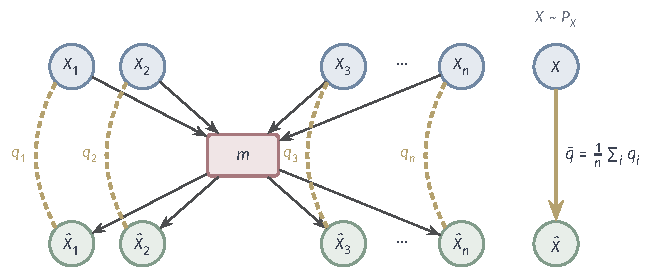
\includegraphics[width=110mm]{figures/07-probability/05-source-coding/tikz/rd-converse-chain/figure.pdf}
  \caption{下界证明的结构。蓝色源符号全部经过红框中的编号$J$（至多$M_n$个值）才到达绿色重构。黄色虚线表示每一对$(X_i,\hat{X}_i)$的条件分布，它是一个单符号测试信道$q_i$；右侧是它们的平均$\bar{q}$，输入仍服从$P_X$。}
  \label{fig:rd-converse-chain}
\end{BookInlineFigure}

\paragraph{第一步：编号限制信息}
$X^{n}\to J\to\hat{X}^{n}$构成Markov链：$\hat{X}^{n}$是$J$的函数，给定$J$后不再依赖$X^{n}$。由第~\ref{chap:information-measures}章的数据处理不等式，后处理不增加信息，
\[
  I(X^{n};\hat{X}^{n})\leq I(X^{n};J)\leq H(J)\leq\log_2M .
\]
第二个不等号是$I(X^{n};J)=H(J)-H(J\mid X^{n})$与条件熵非负，第三个是$J$只取$M$个值。

\paragraph{第二步：拆成单个符号}
把互信息写成源块的熵减去给定重构后的条件熵。信源无记忆，各$X_i$独立，联合熵可加：
\[
  H(X^{n})=\sum_{i=1}^{n}H(X_i).
\]
条件熵用链式法则逐个展开，再用“条件越多熵越小”去掉多余的条件：
\[
  H(X^{n}\mid\hat{X}^{n})=\sum_{i=1}^{n}H(X_i\mid X_1,\dots,X_{i-1},\hat{X}^{n})\leq\sum_{i=1}^{n}H(X_i\mid\hat{X}_i).
\]
两式相减，得到
\[
  I(X^{n};\hat{X}^{n})\geq\sum_{i=1}^{n}\bigl(H(X_i)-H(X_i\mid\hat{X}_i)\bigr)=\sum_{i=1}^{n}I(X_i;\hat{X}_i).
\]

\paragraph{第三步：平均成一个测试信道}
记第$i$个位置的条件分布为
\[
  q_i(\hat{x}\mid x)=\mathbb{P}(\hat{X}_i=\hat{x}\mid X_i=x),
\]
对$p(x)>0$的$x$定义，其余$x$任取一个分布。因为每个$X_i$都服从$P_X$，第$i$对的互信息就是$I(P_X,q_i)$。第$i$个位置的平均失真记为$\Delta_i$，它就是$q_i$在式~\eqref{eq:rd-test-distortion}中的失真。

令$\bar{q}=\frac1n\sum_iq_i$，由引理~\ref{lem:rd-mi-convex}（推广到$n$个信道的凸组合，按$n$归纳），
\[
  \frac1n\sum_{i=1}^{n}I(P_X,q_i)\geq I(P_X,\bar{q}).
\]
失真对测试信道线性，$\bar{q}$的平均失真是$\frac1n\sum_i\Delta_i$。由式~\eqref{eq:rd-block-distortion}，它正是$\Delta$。所以$\bar{q}$在$R(\Delta)$的可行集合中，$I(P_X,\bar{q})\geq R(\Delta)$。

把三步连起来：
\[
  \log_2M\geq I(X^{n};\hat{X}^{n})\geq\sum_{i=1}^{n}I(P_X,q_i)\geq n\,I(P_X,\bar{q})\geq n\,R(\Delta),
\]
这就是式~\eqref{eq:rd-converse}。

\paragraph{从单个码到渐近下界}
设$(R',D)$可达，相应码列的期望失真为$\Delta_n$，$\limsup_n\Delta_n\leq D$。对任意$\varepsilon>0$，$n$充分大时$\Delta_n\leq D+\varepsilon$，由式~\eqref{eq:rd-converse}与$R$非增，
\[
  \frac{\log_2M_n}{n}\geq R(\Delta_n)\geq R(D+\varepsilon).
\]
取上极限得$R'\geq R(D+\varepsilon)$。由定理~\ref{thm:rd-existence}，$R$在$[D_{\min},\infty)$上连续，令$\varepsilon\to0$得$R'\geq R(D)$。所以$R_{\mathrm{op}}(D)\geq R(D)$。

\paragraph{两个假设各用在哪里}
无记忆性用在第二步与第三步：$H(X^{n})=\sum_iH(X_i)$需要独立，$I(X_i;\hat{X}_i)=I(P_X,q_i)$需要每个$X_i$的分布都是$P_X$。可分失真用在第三步的最后：$\bar{q}$的失真等于块失真，靠的是块失真等于逐符号失真的平均。

去掉无记忆性，单符号的$R(D)$就不再是正确答案。设$Y\sim\operatorname{Bern}(0.3)$，令$X_1=X_2=\dots=X_n=Y$。每个$X_i$的分布仍是$\operatorname{Bern}(0.3)$，单符号的$R(0)$仍是$h_2(0.3)\approx0.881$。可是整块只有两种可能，用$1$\,bit传送$Y$就能零失真重构，码率$1/n\to0$。第二步中
\[
  H(X^{n})=h_2(0.3),\qquad \sum_{i=1}^{n}H(X_i)=n\,h_2(0.3),
\]
前者远小于后者，链条在这里断开。带记忆的信源需要按块定义信息量再取极限，本章不讨论。

\subsection{可达的码率}
\label{sec:rd-achievability}

下界说码率不能低于$R(D)$。反方向要构造码。直接设计最优码本很难，下面的办法是随机撒点：按最优测试信道的重构边缘独立地生成很多码字，证明平均而言总有一个码字离源块足够近，再由平均推出确定的好码本存在。

\paragraph{为什么随机码本能覆盖}
取达到$R(D)$的测试信道$q$（定理~\ref{thm:rd-existence}保证存在），它的重构边缘为$r=r_q$，$I=I(P_X,q)=R(D)$。对一个典型的源块$x^{n}$，随机抽一个码字$Y^{n}$，各分量独立服从$r$，它“恰好与$x^{n}$配成像是由$q$产生的一对”的概率有多大？

对一对$(x,\hat{x})$，记\term{信息密度}（information density）
\begin{equation}
  \imath(x,\hat{x})=\log_2\frac{q(\hat{x}\mid x)}{r(\hat{x})},\qquad
  \imath_n(x^{n},\hat{x}^{n})=\sum_{i=1}^{n}\imath(x_i,\hat{x}_i),
  \label{eq:rd-information-density}
\end{equation}
只在$q(\hat{x}\mid x)>0$处定义。按联合分布$p(x)q(\hat{x}\mid x)$取期望，由式~\eqref{eq:rd-test-information}，$\mathbb{E}\,\imath(X,\hat{X})=I$。$\imath_n$越大，块对$(x^{n},\hat{x}^{n})$在$q$下比在“$\hat{x}^{n}$与$x^{n}$无关”时越可能出现，倍数是$2^{\imath_n}$。

若$(X_i,\hat{X}_i)$独立地按$p(x)q(\hat{x}\mid x)$产生，大数律使$\frac1n\imath_n$集中在$I$附近，图~\ref{fig:rd-info-density}展示了这种集中。于是“像是由$q$产生的”块对，其$\imath_n$约为$nI$，从$r^{n}$中独立抽到这样的$\hat{x}^{n}$的概率约为$2^{-nI}$。要有把握至少抽中一个，码字数应超过$2^{nI}$，也就是码率略高于$I=R(D)$。

\begin{BookInlineFigure}
  \centering
  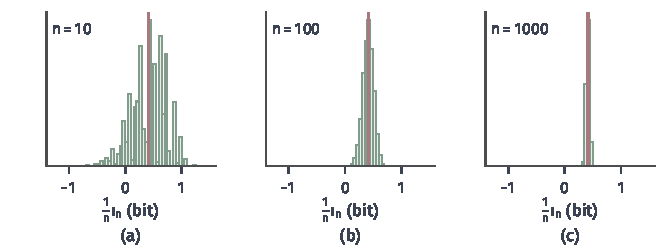
\includegraphics[width=112mm]{figures/07-probability/05-source-coding/matplotlib/rd-info-density/figure.pdf}
  \caption{$\operatorname{Bern}(0.3)$信源、Hamming失真、$D=0.1$的最优联合分布下，每符号信息密度$\frac1n\imath_n$的直方图（绿），块长$n=10,100,1000$，各$20000$个块，随机种子$722$。单个符号的$\imath$只取$0.363$、$-2.807$、$-1.585$、$1.585$四个值；红线是均值$I=R(0.1)\approx0.412$。$n=1000$时样本标准差约为$0.029$。}
  \label{fig:rd-info-density}
\end{BookInlineFigure}

下面把这个估计写成不等式。对$\gamma>0$与$D'\geq0$，令
\[
  \mathcal{A}=\Bigl\{(x^{n},\hat{x}^{n}):\ q^{n}(\hat{x}^{n}\mid x^{n})>0,\ \imath_n(x^{n},\hat{x}^{n})\leq\log_2\gamma,\ d_n(x^{n},\hat{x}^{n})\leq D'\Bigr\},
\]
其中$q^{n}$是$q$逐符号作用于整块的条件概率，即各分量$q(\hat{x}_i\mid x_i)$的乘积。$\mathcal{A}$中的块对失真达标，信息密度又不过大，称为\term{失真典型集}（distortion-typical set）。对固定的$x^{n}$，把与它配成$\mathcal{A}$中块对的重构块全体记为$\mathcal{A}(x^{n})$。

\begin{lemma}[随机码本的覆盖]
\label{lem:rd-covering}
设码字$C_1,\dots,C_M$相互独立，各分量独立服从$r$，并与$X^{n}$独立。令$(X^{n},\hat{X}^{n})$按$\prod_ip(x_i)q(\hat{x}_i\mid x_i)$分布。则
\begin{equation}
  \mathbb{P}\bigl(\text{没有}C_m\in\mathcal{A}(X^{n})\bigr)\leq\mathbb{P}\bigl((X^{n},\hat{X}^{n})\notin\mathcal{A}\bigr)+\mathrm{e}^{-M/\gamma}.
  \label{eq:rd-covering}
\end{equation}
\end{lemma}

\begin{proof}
固定$x^{n}$，令
\[
  g(x^{n})=\sum_{\hat{x}^{n}\in\mathcal{A}(x^{n})}q^{n}(\hat{x}^{n}\mid x^{n}),
\]
它是按测试信道重构时落入$\mathcal{A}(x^{n})$的概率。对$\hat{x}^{n}\in\mathcal{A}(x^{n})$，由式~\eqref{eq:rd-information-density}，
\[
  r^{n}(\hat{x}^{n})=q^{n}(\hat{x}^{n}\mid x^{n})\,2^{-\imath_n(x^{n},\hat{x}^{n})}\geq\frac{1}{\gamma}\,q^{n}(\hat{x}^{n}\mid x^{n}),
\]
其中$r^{n}(\hat{x}^{n})=\prod_ir(\hat{x}_i)$。对$\mathcal{A}(x^{n})$求和，单个码字落入$\mathcal{A}(x^{n})$的概率至少是$g(x^{n})/\gamma$。

$M$个码字独立，全部落空的概率是
\[
  \Bigl(1-\mathbb{P}\bigl(C_1\in\mathcal{A}(x^{n})\bigr)\Bigr)^{M}\leq\Bigl(1-\frac{g(x^{n})}{\gamma}\Bigr)^{M}\leq\exp\Bigl(-\frac{M\,g(x^{n})}{\gamma}\Bigr),
\]
最后一步用了$1-u\leq\mathrm{e}^{-u}$。

再把指数关于$g$放大成线性函数。对$c\geq0$，$t\mapsto\mathrm{e}^{-ct}$在$[0,1]$上凸，图像在两端点连线之下：
\[
  \mathrm{e}^{-ct}\leq(1-t)+t\,\mathrm{e}^{-c}\leq1-t+\mathrm{e}^{-c},\qquad t\in[0,1].
\]
取$c=M/\gamma$，$t=g(x^{n})$，全部落空的概率至多为$1-g(x^{n})+\mathrm{e}^{-M/\gamma}$。

最后对$x^{n}$按$P_X^{n}$平均。$1-g(X^{n})$的期望正是$(X^{n},\hat{X}^{n})\notin\mathcal{A}$的概率，于是得到式~\eqref{eq:rd-covering}。
\end{proof}

式~\eqref{eq:rd-covering}右端两项各有分工。第一项是测试信道本身“不典型”的概率，由大数律控制；第二项是码字太少、撒网不够密的代价，只要$M$远大于$\gamma\approx2^{nI}$就可忽略。

\begin{theorem}[可达性]
\label{thm:rd-achievability}
在本节设定下，对$D\geq D_{\min}$与任意$R'>R(D)$，$(R',D)$可达。于是$R_{\mathrm{op}}(D)\leq R(D)$。
\end{theorem}

\begin{proof}
取$\delta>0$，令$I=R(D)$，$q$为达到$R(D)$的测试信道，$\mathbb{E}_qd\leq D$。下面分四步。

\emph{码本大小。}令$\gamma_n=2^{n(I+\delta)}$，$M_n=\lceil2^{n(I+2\delta)}\rceil$，$D'=D+\delta$。码率满足
\[
  \frac{\log_2M_n}{n}\leq\frac{\log_2\bigl(2^{n(I+2\delta)}+1\bigr)}{n}\to I+2\delta .
\]

\emph{覆盖失败的概率。}$(X_i,\hat{X}_i)$独立同分布，$\imath(X_i,\hat{X}_i)$只取有限个值，均值为$I$；$d(X_i,\hat{X}_i)$有界，均值不超过$D$。由第~\ref{chap:laws-of-large-numbers}章的弱大数律，
\[
  \mathbb{P}\Bigl(\frac1n\imath_n>I+\delta\Bigr)\to0,\qquad \mathbb{P}\bigl(d_n>D+\delta\bigr)\to0 .
\]
所以式~\eqref{eq:rd-covering}的第一项趋于零。第二项中$M_n/\gamma_n\geq2^{n\delta}$，故
\[
  \mathrm{e}^{-M_n/\gamma_n}\leq\exp(-2^{n\delta})\to0 .
\]记右端为$\varepsilon_n$，$\varepsilon_n\to0$。

\emph{随机码的平均失真。}用最近码字编码器。只要有一个$C_m\in\mathcal{A}(X^{n})$，最近码字的失真就不超过$D+\delta$；否则失真不超过$d_{\max}$。对源与码本一起取期望，
\[
  \mathbb{E}\bigl[d_n(X^{n},\hat{X}^{n})\bigr]\leq D+\delta+d_{\max}\,\varepsilon_n .
\]

\emph{从随机码本到确定码本。}左端是对随机码本取平均后的期望失真，平均值不超过某个数，至少有一个码本的期望失真不超过这个数。于是对每个充分大的$n$，存在确定的$(n,M_n)$码，期望失真不超过$D+\delta+d_{\max}\varepsilon_n$。对较小的$n$随便取一个码，不影响上极限。这说明$(I+2\delta,D+\delta)$可达。

$\delta$可以任意小。给定$R'>I$，对一切满足$I+2\delta\leq R'$的$\delta$，$(R',D+\delta)$都可达。下面的对角线论证说明$(R',D)$也可达。
\end{proof}

\paragraph{边界点的极限处理}
设对每个$k$，$(R',D+\tfrac1k)$可达，相应的码列为$\mathcal{C}^{(k)}$。由上极限的定义，存在$N_k$，使$n\geq N_k$时$\mathcal{C}^{(k)}$中块长为$n$的码满足
\[
  \frac{\log_2M_n}{n}\leq R'+\frac1k,\qquad \mathbb{E}d_n\leq D+\frac2k .
\]
可以取$N_1<N_2<\cdots$。对$N_k\leq n<N_{k+1}$，块长$n$时使用$\mathcal{C}^{(k)}$中的码。$n\to\infty$时所用的$k$也趋于无穷，所以新码列满足式~\eqref{eq:rd-achievable}，$(R',D)$可达。可达区域在这个意义下是闭的。

至此$R_{\mathrm{op}}(D)\leq R(D)$，与第~\ref{sec:rd-converse}节的下界合起来，定理~\ref{thm:rd-coding}得证。在$D=D_{\min}$处，下界用到了$R$在端点的右连续，可达性则靠这里的极限处理；两边都不要求在端点处有特别的构造。

\paragraph{有限块长与计算代价}
定理只保证极限。先给极限一个记号：由定理~\ref{thm:rd-zero-rate}，$R$在$[D_{\min},D_{\max}]$上严格递减，它的反函数记为$D(R)$，称为\term{失真率函数}（distortion-rate function），表示码率为$R$时能达到的最小失真。雨天记录中$D(0.5)\approx0.0742$，即$R(D)=0.5$的解。

图~\ref{fig:rd-finite-codes}(a)用穷举给出$n\leq4$时每种码本大小下最好的码，它们都在曲线上方不远处，码率$\tfrac12$时最好的失真从$n=2$的$0.15$降到$n=4$的约$0.136$，离$D(0.5)$仍有距离。图~\ref{fig:rd-finite-codes}(b)是按证明构造的随机码本：码率固定为$\tfrac12$，块长到$36$时平均失真约为$0.097$，仍明显高于极限。

\begin{BookInlineFigure}
  \centering
  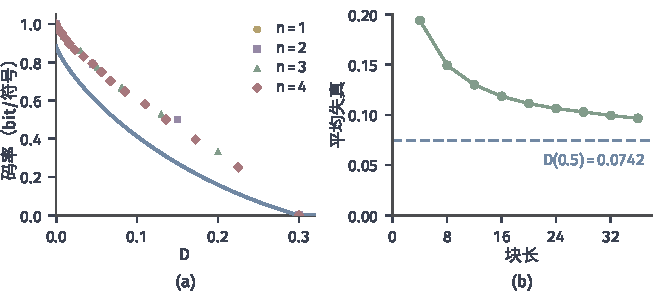
\includegraphics[width=112mm]{figures/07-probability/05-source-coding/matplotlib/rd-finite-codes/figure.pdf}
  \caption{$\operatorname{Bern}(0.3)$信源与Hamming失真下的有限块长码。(a)对$n=1,2,3,4$穷举全部码本，每种码本大小$M$下期望失真最小的码（不同颜色与形状），横坐标为失真，纵坐标为$\log_2M/n$；蓝线是$R(D)$。(b)码率$\tfrac12$的随机码本，码字各分量独立服从$\operatorname{Bern}(0.265)$（码率$\tfrac12$对应的最优重构边缘），最近码字编码；每个$n$用$40$个码本、每个码本$250$个源块估计平均失真，随机种子$722$。蓝色虚线是$D(0.5)\approx0.0742$。}
  \label{fig:rd-finite-codes}
\end{BookInlineFigure}

收敛慢的原因可以从证明中看出：$\frac1n\imath_n$与$d_n$的波动按$n^{-1/2}$缩小，要让它们都落在$\delta$以内，$n$要远大于$\delta^{-2}$。计算上，最近码字编码要在$2^{nR}$个码字中搜索，$n=36$、$R=\tfrac12$时已有约$2.6\times10^{5}$个码字。证明给出的是存在性，构造搜索代价低的好码是另一个问题，本章不讨论。


\section{可解析的模型}
\label{sec:rd-analytic}

编码定理把问题交还给式~\eqref{eq:rd-information-rd}的优化。少数模型可以精确求解，办法都是两步：先证明一个对所有满足失真约束的测试信道都成立的互信息下界，再构造一个测试信道使下界取等号。下界说“不可能更省”，构造说“确实能做到”，两者相遇处就是$R(D)$。

构造时常常反过来想：不直接写$q(\hat{x}\mid x)$，而是先给出$\hat{X}$的分布，再说明$X$怎样由$\hat{X}$加上一个独立的“误差”得到。这种从重构到源的描述称为\term{反向测试信道}（backward test channel）。只要它产生的$X$恰好服从给定的源分布，对$X$取条件就得到一个普通的测试信道。

\subsection{二元信源}
\label{sec:rd-binary}

开头的雨天记录现在可以算到底。设$X\sim\operatorname{Bern}(p)$，失真为Hamming失真。交换符号$0$与$1$不改变问题，所以不妨设$p\leq\tfrac12$。由第~\ref{sec:rd-feasible-range}节，$D_{\min}=0$，$D_{\max}=p$，零码率时一律输出更常见的$0$。

\begin{theorem}[二元信源的率失真函数]
\label{thm:rd-binary}
设$X\sim\operatorname{Bern}(p)$，$0\leq p\leq\tfrac12$，失真为式~\eqref{eq:rd-hamming}。则
\begin{equation}
  R(D)=\begin{cases}
    h_2(p)-h_2(D), & 0\leq D\leq p,\\
    0, & D\geq p.
  \end{cases}
  \label{eq:rd-binary}
\end{equation}
\end{theorem}

\begin{proof}
$D\geq p$时由定理~\ref{thm:rd-zero-rate}得$R(D)=0$。下面设$0\leq D<p$，于是$p>0$。

\emph{下界。}任取满足$\mathbb{E}d\leq D$的测试信道，令$E=X\oplus\hat{X}$为模$2$和，$E=1$表示重构出错，$\mathbb{P}(E=1)=\mathbb{E}d\leq D$。给定$\hat{X}$时，$X\mapsto X\oplus\hat{X}$是一一对应，条件熵不变，所以
\[
  H(X\mid\hat{X})=H(E\mid\hat{X})\leq H(E)=h_2\bigl(\mathbb{P}(E=1)\bigr)\leq h_2(D).
\]
最后一步用了$h_2$在$[0,\tfrac12]$上递增，以及$\mathbb{P}(E=1)\leq D<\tfrac12$。于是
\[
  I(X;\hat{X})=H(X)-H(X\mid\hat{X})\geq h_2(p)-h_2(D).
\]

\emph{达到下界。}令
\[
  r=\frac{p-D}{1-2D}.
\]
由$0\leq D<p\leq\tfrac12$，分子与分母都为正；又$p\leq\tfrac12<1-D$，所以$p-D<1-2D$，$r\in(0,1)$。取相互独立的$\hat{X}\sim\operatorname{Bern}(r)$与$Z\sim\operatorname{Bern}(D)$，令$X=\hat{X}\oplus Z$。

$X=1$当且仅当$\hat{X}$与$Z$恰有一个为$1$，
\[
  \mathbb{P}(X=1)=r(1-D)+(1-r)D=D+r(1-2D)=p ,
\]
所以$X$恰好服从源分布，$(X,\hat{X})$的联合分布给出一个测试信道。它的失真是$\mathbb{P}(X\neq\hat{X})=\mathbb{P}(Z=1)=D$。$Z$与$\hat{X}$独立，
\[
  I(X;\hat{X})=H(X)-H(X\mid\hat{X})=h_2(p)-H(Z\mid\hat{X})=h_2(p)-h_2(D),
\]
与下界相等。
\end{proof}

下界的证明说明了等号何时成立：错误指示$E$必须与$\hat{X}$独立，并且错误率恰为$D$。构造的反向测试信道正好满足这两点。图~\ref{fig:rd-binary-test-channels}(a)画出$p=0.3$、$D=0.1$时的反向信道：$\hat{X}\sim\operatorname{Bern}(0.25)$，再以$0.1$的概率翻转，得到$\operatorname{Bern}(0.3)$。

用Bayes公式换回从$X$到$\hat{X}$的方向。$X=0$而$\hat{X}=1$需要$\hat{X}=1$且$Z=1$；$X=1$而$\hat{X}=0$需要$\hat{X}=0$且$Z=1$。于是
\[
  \begin{aligned}
  q(1\mid0)&=\frac{rD}{1-p}=\frac{0.25\times0.1}{0.7}=\frac1{28},\\
  q(0\mid1)&=\frac{(1-r)D}{p}=\frac{0.75\times0.1}{0.3}=\frac14 ,
  \end{aligned}
\]
这就是第~\ref{sec:rd-test-channels}节第三个测试信道，图~\ref{fig:rd-binary-test-channels}(b)画出了它。由式~\eqref{eq:rd-binary}，
\[
  R(0.1)=h_2(0.3)-h_2(0.1)\approx0.8813-0.4690=0.4123 .
\]

\begin{BookInlineFigure}
  \centering
  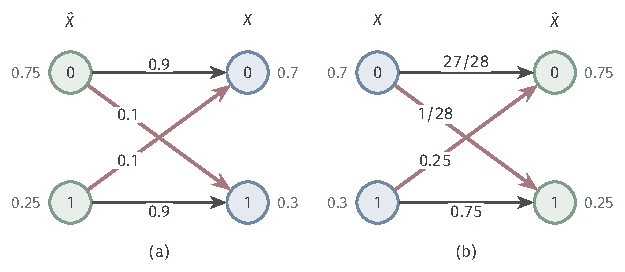
\includegraphics[width=106mm]{figures/07-probability/05-source-coding/tikz/rd-binary-test-channels/figure.pdf}
  \caption{$X\sim\operatorname{Bern}(0.3)$、Hamming失真、$D=0.1$的最优测试信道。(a)反向形式：绿色的$\hat{X}\sim\operatorname{Bern}(0.25)$经过独立的翻转（红箭头，概率$0.1$）得到蓝色的$X$，节点旁的数是边缘概率。(b)由Bayes公式得到的正向形式$q(\hat{x}\mid x)$，罕见符号$1$被改错的概率$\tfrac14$远大于常见符号$0$的$\tfrac1{28}$。}
  \label{fig:rd-binary-test-channels}
\end{BookInlineFigure}

开头的问题有了答案：允许错$10\%$，每天只需约$0.412$\,bit，不到无损所需$0.881$\,bit的一半，远少于按比例打折的$0.881\times0.9\approx0.793$。第~\ref{sec:rd-block-model}节中要求每一块都不超过$10\%$错误时至少需要$0.531$\,bit；期望失真要求允许少数块错得多，于是更省。

\paragraph{源概率与端点}
图~\ref{fig:rd-binary-curves}画出三个源概率下的曲线，可以对照式~\eqref{eq:rd-binary}逐项检查。
\begin{itemize}
  \item $D=0$时$R(0)=h_2(p)=H(X)$，回到无损编码的熵。
  \item 曲线在$D_{\max}=p$处降到零，零码率失真由源概率决定：$p=0.1$时一律猜$0$只错$10\%$，$p=\tfrac12$时要错一半。
  \item 均匀信源$p=\tfrac12$时$R(D)=1-h_2(D)$，这只是$p$的一个取值，曲线最高，因为每个符号最难预测。
  \item 退化情形$p=0$时信源是常数$0$，$D_{\max}=0$，$R\equiv0$；这时$h_2(p)-h_2(D)$在$D>0$时为负，公式只能在$0\leq D\leq p$上使用。
\end{itemize}

曲线的斜率是$R'(D)=-h_2'(D)=-\log_2\frac{1-D}{D}$，$D\downarrow0$时趋于$-\infty$。允许极少量的错误就能省下相当多的码率，这是有损压缩在低失真端最划算的原因；越往后，每多容忍一点失真省下的码率越少。

\begin{BookInlineFigure}
  \centering
  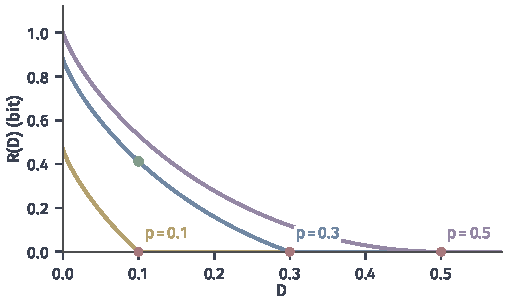
\includegraphics[width=86mm]{figures/07-probability/05-source-coding/matplotlib/rd-binary-curves/figure.pdf}
  \caption{$\operatorname{Bern}(p)$信源在Hamming失真下的$R(D)$，$p=0.1$（黄）、$0.3$（蓝）、$0.5$（紫）。红点是零码率失真$D_{\max}=p$，曲线在纵轴上的截距是$h_2(p)$。绿点是贯穿例子$(0.1,0.4123)$。}
  \label{fig:rd-binary-curves}
\end{BookInlineFigure}

\subsection{高斯信源}
\label{sec:rd-gaussian}

开头的第二个问题涉及实值信源与平方失真。这里重构值连续变化，第~\ref{sec:rd-coding-theorem}节的有限字母表证明不能直接搬用；我们先在信息率失真函数的层面上求解，再说明编码定理在这里的地位。计算需要一个关于微分熵的不等式，它也会在第~\ref{chap:gaussian-channel-capacity}章计算高斯信道容量时用到。

本小节沿用第~\ref{chap:information-measures}章的微分熵，换成以bit计：对有密度$f$的实值随机变量，
\[
  h(X)=-\int_{\mathbb{R}}f(x)\log_2f(x)\,\mathrm{d}x ,
\]
前提是这个积分有意义。KL散度同样以bit计，即在第~\ref{chap:distribution-comparison}章的定义中把$\ln$换成$\log_2$，它仍然非负，且为零当且仅当两个分布相同。

\subsubsection{高斯分布的熵上界}
\label{sec:rd-gaussian-entropy}

方差固定时，哪种分布的不确定性最大？图~\ref{fig:rd-gaussian-entropy}中三个密度均值都是$0$、方差都是$1$。均匀分布把质量平铺在$[-\sqrt3,\sqrt3]$上，Laplace分布尖峰更高、尾部更厚，高斯分布介于两者之间。它们的微分熵分别是
\[
  \log_2(2\sqrt3)\approx1.792,\qquad \log_2(\sqrt2\,\mathrm{e})\approx1.943,\qquad \frac12\log_2(2\pi\mathrm{e})\approx2.047 ,
\]
第二个用了Laplace分布$\operatorname{Laplace}(0,b)$的方差$2b^{2}=1$与熵$\log_2(2\mathrm{e}b)$。高斯最大，这不是巧合。

\begin{BookInlineFigure}
  \centering
  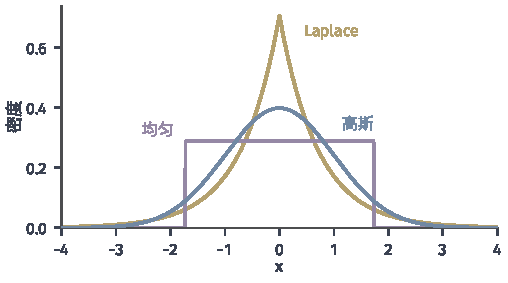
\includegraphics[width=86mm]{figures/07-probability/05-source-coding/matplotlib/rd-gaussian-entropy/figure.pdf}
  \caption{均值为$0$、方差为$1$的三个密度：标准高斯（蓝，$h\approx2.047$\,bit）、$\operatorname{Laplace}(0,1/\sqrt2)$（黄，$h\approx1.943$\,bit）、$[-\sqrt3,\sqrt3]$上的均匀分布（紫，$h\approx1.792$\,bit）。三个熵值也用数值积分核对过。}
  \label{fig:rd-gaussian-entropy}
\end{BookInlineFigure}

\begin{theorem}[固定方差的熵上界]
\label{thm:rd-gaussian-max-entropy}
设实值随机变量$X$有密度$f$，均值为$\mu$，方差$\sigma^{2}\in(0,\infty)$。则定义$h(X)$的积分有意义，取值于$[-\infty,\infty)$，并且
\begin{equation}
  h(X)\leq\frac12\log_2(2\pi\mathrm{e}\sigma^{2}),
  \label{eq:rd-gaussian-max-entropy}
\end{equation}
等号成立当且仅当$X\sim\mathcal{N}(\mu,\sigma^{2})$。
\end{theorem}

\begin{proof}
取同均值、同方差的高斯密度作参考，
\[
  g(x)=\frac{1}{\sqrt{2\pi\sigma^{2}}}\exp\Bigl(-\frac{(x-\mu)^{2}}{2\sigma^{2}}\Bigr).
\]
先算$-\log_2g$在$f$下的期望。由$g$的表达式，
\[
  -\log_2g(x)=\frac12\log_2(2\pi\sigma^{2})+(\log_2\mathrm{e})\frac{(x-\mu)^{2}}{2\sigma^{2}},
\]
它是$x$的二次函数，在$f$下可积。由$\mathbb{E}(X-\mu)^{2}=\sigma^{2}$，
\[
  -\int f\log_2g\,\mathrm{d}x=\frac12\log_2(2\pi\sigma^{2})+\frac{\log_2\mathrm{e}}{2}=\frac12\log_2(2\pi\mathrm{e}\sigma^{2}).
\]

再看KL散度的被积函数$f\log_2(f/g)$（在$f>0$处）。由$\ln t\geq1-1/t$，
\[
  f\ln\frac{f}{g}\geq f-g ,
\]
所以它的负部不超过$g$，可积。于是KL散度
\[
  D_{\mathrm{KL}}(f\Vert g)=\int f\log_2\frac{f}{g}\,\mathrm{d}x
\]
有意义，取值于$[0,\infty]$。

在$f>0$处写$f\log_2f=f\log_2(f/g)+f\log_2g$。右端第一项负部可积，第二项可积，所以$f\log_2f$的负部可积，$\int f\log_2f\,\mathrm{d}x$有意义且大于$-\infty$。这说明$h(X)$有意义，取值于$[-\infty,\infty)$，并且
\[
  h(X)=-\int f\log_2\frac{f}{g}\,\mathrm{d}x-\int f\log_2g\,\mathrm{d}x=\frac12\log_2(2\pi\mathrm{e}\sigma^{2})-D_{\mathrm{KL}}(f\Vert g).
\]
KL散度非负，得到式~\eqref{eq:rd-gaussian-max-entropy}。等号成立当且仅当$D_{\mathrm{KL}}(f\Vert g)=0$，即$f=g$几乎处处，也就是$X\sim\mathcal{N}(\mu,\sigma^{2})$。
\end{proof}

证明里的关键是：$-\log_2g$只是$x$的二次函数，它在任何同方差分布下的平均都一样。于是“$f$的熵比高斯少多少”恰好就是$f$与高斯的KL散度。条件中的方差有限保证了这个平均有限；$h(X)$可以是$-\infty$（例如密度在某些点附近极度集中），不等式仍然成立，只是没有信息量。没有方差限制时，微分熵没有上界：$\operatorname{Unif}(0,a)$的熵$\log_2a$随$a$无限增大。

\subsubsection{高斯率失真函数}
\label{sec:rd-gaussian-rd}

设$X\sim\mathcal{N}(\mu,\sigma^{2})$，$\sigma^{2}>0$，失真为平方误差。测试信道是从$\mathbb{R}$到$\mathbb{R}$的Markov核，$R(D)$仍按式~\eqref{eq:rd-information-rd}定义，互信息是联合分布相对边缘乘积的KL散度，可以为$+\infty$。

\begin{theorem}[高斯信源的率失真函数]
\label{thm:rd-gaussian}
在上述设定下，
\begin{equation}
  R(D)=\begin{cases}
    \dfrac12\log_2\dfrac{\sigma^{2}}{D}, & 0<D<\sigma^{2},\\
    0, & D\geq\sigma^{2},
  \end{cases}
  \label{eq:rd-gaussian}
\end{equation}
且$R(0)=+\infty$。单位是bit每个实值源符号。
\end{theorem}

\begin{proof}
把$X$与$\hat{X}$同时减去$\mu$，平方误差与互信息都不变，所以不妨设$\mu=0$。$D\geq\sigma^{2}$时恒输出$0$，失真为$\mathbb{E}X^{2}=\sigma^{2}\leq D$，互信息为零。下面设$0<D<\sigma^{2}$，分下界与达到两部分。

\emph{下界的分解。}任取满足$\mathbb{E}(X-\hat{X})^{2}\leq D$的联合分布。若$I(X;\hat{X})=+\infty$无需证明，下设它有限。这时联合分布对$P_X\otimes P_{\hat{X}}$绝对连续，记Radon–Nikodym导数为$\lambda(x,\hat{x})$，则互信息是$\log_2\lambda(X,\hat{X})$的期望。$P_X$有密度$f=\varphi_{\sigma^{2}}$（方差为$\sigma^{2}$的零均值高斯密度），所以给定$\hat{X}=\hat{x}$时$X$的条件分布有密度$p(x\mid\hat{x})=\lambda(x,\hat{x})f(x)$，并且
\[
  I(X;\hat{X})=\mathbb{E}\Bigl[\log_2\frac{p(X\mid\hat{X})}{f(X)}\Bigr].
\]

\emph{条件高斯参考。}引入一个“猜测”的条件密度$w(x\mid\hat{x})=\varphi_D(x-\hat{x})$，即以$\hat{x}$为中心、方差为$D$的高斯密度。把对数拆成两项：
\[
  \log_2\frac{p(X\mid\hat{X})}{f(X)}=\log_2\frac{p(X\mid\hat{X})}{w(X\mid\hat{X})}+\log_2\frac{w(X\mid\hat{X})}{f(X)} .
\]
第二项写开是
\[
  \frac12\log_2\frac{\sigma^{2}}{D}-\frac{\log_2\mathrm{e}}{2}\Bigl(\frac{(X-\hat{X})^{2}}{D}-\frac{X^{2}}{\sigma^{2}}\Bigr),
\]
由$\mathbb{E}X^{2}=\sigma^{2}$与$\mathbb{E}(X-\hat{X})^{2}\leq D$，它可积，期望至少为
\[
  \frac12\log_2\frac{\sigma^{2}}{D}-\frac{\log_2\mathrm{e}}{2}\,(1-1)=\frac12\log_2\frac{\sigma^{2}}{D}.
\]

\emph{条件KL非负。}左端与第二项都可积，所以第一项可积。对$\hat{X}$取条件，第一项的条件期望是条件分布$p(\cdot\mid\hat{X})$相对参考$w(\cdot\mid\hat{X})$的KL散度，非负；再对$\hat{X}$平均仍非负。于是
\[
  I(X;\hat{X})\geq\frac12\log_2\frac{\sigma^{2}}{D}.
\]

\emph{达到下界。}取相互独立的$\hat{X}\sim\mathcal{N}(0,\sigma^{2}-D)$与$Z\sim\mathcal{N}(0,D)$，令$X=\hat{X}+Z$。独立高斯之和仍是高斯，$X\sim\mathcal{N}(0,\sigma^{2})$，失真$\mathbb{E}(X-\hat{X})^{2}=\mathbb{E}Z^{2}=D$。这时条件密度$p(\cdot\mid\hat{x})$恰是参考$w(\cdot\mid\hat{x})$，第一项恒为零；第二项中$\mathbb{E}(X-\hat{X})^{2}=D$，期望恰为$\tfrac12\log_2(\sigma^{2}/D)$。下界取到。

\emph{零失真。}$D=0$时可行的联合分布必须满足$\hat{X}=X$几乎必然，联合分布集中在对角线上，而$P_X\otimes P_X$给对角线的概率为零，联合分布不对乘积绝对连续，互信息为$+\infty$。
\end{proof}

\paragraph{改写成熵差}
当相关的微分熵都有限时，上面的下界有一个更直观的读法。此时$I(X;\hat{X})=h(X)-h(X\mid\hat{X})$。给定$\hat{X}$后，$X$与误差$X-\hat{X}$只差一个已知的平移，条件熵相同；条件化不增加熵；再对误差用定理~\ref{thm:rd-gaussian-max-entropy}，其方差不超过$\mathbb{E}(X-\hat{X})^{2}\leq D$：
\[
  h(X\mid\hat{X})=h(X-\hat{X}\mid\hat{X})\leq h(X-\hat{X})\leq\frac12\log_2(2\pi\mathrm{e}D).
\]
于是
\[
  I(X;\hat{X})\geq\frac12\log_2(2\pi\mathrm{e}\sigma^{2})-\frac12\log_2(2\pi\mathrm{e}D)=\frac12\log_2\frac{\sigma^{2}}{D},
\]
与定理一致：重构后剩下的不确定性，至多是一个方差为$D$的高斯误差的不确定性。

这个读法要求每个熵项都有意义且有限，否则会出现“无穷减无穷”；例如$\hat{X}$只取有限个值时，给定$\hat{X}$后$X$的条件熵要逐值核对。上面的证明只用条件KL，不需要这些前提，两者的数学内容相同：熵上界的证明本身就是相对高斯参考的KL非负。

\paragraph{几何图景}
达到下界的反向测试信道是$X=\hat{X}+Z$，$\hat{X}$与$Z$独立。在均方意义下，独立且零均值就是正交，于是$\sigma^{2}=(\sigma^{2}-D)+D$是一个勾股关系，图~\ref{fig:rd-gaussian-geometry}画出了这个直角三角形。最优重构是源的一个“缩短的影子”：它的方差只有$\sigma^{2}-D$，不是$\sigma^{2}$。

从$X$看，$(X,\hat{X})$是联合高斯，$\operatorname{Cov}(X,\hat{X})=\sigma^{2}-D$。记$a=1-D/\sigma^{2}$，由二元高斯的条件分布，
\[
  \mathbb{E}[\hat{X}\mid X]=aX,\qquad \operatorname{Var}(\hat{X}\mid X)=(\sigma^{2}-D)-\frac{(\sigma^{2}-D)^{2}}{\sigma^{2}}=aD .
\]
所以正向测试信道是$q(\cdot\mid x)=\mathcal{N}(ax,aD)$：先把$x$向$0$收缩到$ax$，再加上方差为$aD$的独立噪声。

\begin{BookInlineFigure}
  \centering
  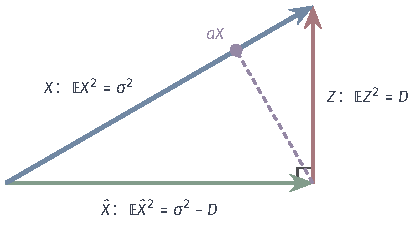
\includegraphics[width=72mm]{figures/07-probability/05-source-coding/tikz/rd-gaussian-geometry/figure.pdf}
  \caption{高斯最优测试信道的均方几何，$\sigma^{2}=1$，$D=\tfrac14$。向量长度表示均方根：绿色$\hat{X}$与红色误差$Z$独立因而正交，合成蓝色的$X$。紫点是$\hat{X}$在$X$方向上的投影$aX$，$a=1-D/\sigma^{2}=\tfrac34$，紫色虚线垂直于$X$。}
  \label{fig:rd-gaussian-geometry}
\end{BookInlineFigure}

\paragraph{各个区间的码率}
式~\eqref{eq:rd-gaussian}的三段各有含义。
\begin{itemize}
  \item $0<D<\sigma^{2}$时，反解得失真率函数$D(R)=\sigma^{2}2^{-2R}$：每多$1$\,bit，均方误差降为四分之一。$\sigma^{2}=1$、$D=\tfrac14$时恰需$1$\,bit。
  \item $D\geq\sigma^{2}$时不需要描述，输出均值即可，零码率失真就是方差。
  \item $D\downarrow0$时$R(D)\to\infty$：连续取值的信源不能用有限码率精确描述，这与有限字母表上$R(0)=H(X)$的情形不同。
\end{itemize}
均值$\mu$只影响平移，不改变码率。退化的$\sigma^{2}=0$是确定的源$X=\mu$，对一切$D\geq0$有$R(D)=0$，公式~\eqref{eq:rd-gaussian}不适用。

\paragraph{编码定理与有限量化器}
定理~\ref{thm:rd-gaussian}是关于信息率失真函数的结论。要说$R(D)$也是高斯信源在平方失真下的最低渐近码率，还需要把编码定理推广到连续字母表与无界失真：可以先把源与重构离散化、截断尾部，在有限字母表上用第~\ref{sec:rd-coding-theorem}节的定理，再控制离散化与尾部带来的误差。结论成立，但证明较长，读者可查阅~\scite{math-cover2006information}。

承认这一点，就能回答开头的第二个问题。图~\ref{fig:rd-gaussian-quantizers}对标准高斯信源比较几类方案。码率为$1$\,bit时，极限是$D(1)=0.25$，而第~\ref{chap:quantization}章的两点最优量化器只做到$1-2/\pi\approx0.363$。反过来看，失真$0.363$只需
\[
  R(0.363)=\frac12\log_2\frac{1}{0.363}\approx0.730
\]
bit，逐个量化多用了约$0.27$\,bit。四点、八点、十六点的Lloyd–Max量化器与极限之间也一直有差距。

\begin{BookInlineFigure}
  \centering
  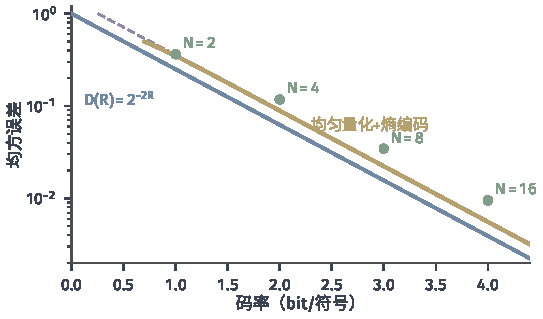
\includegraphics[width=92mm]{figures/07-probability/05-source-coding/matplotlib/rd-gaussian-quantizers/figure.pdf}
  \caption{标准高斯信源在平方失真下的码率与均方误差，纵轴为对数刻度。蓝线是$D(R)=2^{-2R}$。绿点是$N=2,4,8,16$个重构值的Lloyd–Max量化器，码率取定长索引的$\log_2N$。黄线是步长从$3$减小到$0.1$的均匀量化器（重构取区间条件均值），码率取索引的熵，即理想无损压缩索引后的平均长度。紫色虚线是蓝线向右平移$\tfrac12\log_2\frac{\pi\mathrm{e}}{6}\approx0.2546$\,bit。}
  \label{fig:rd-gaussian-quantizers}
\end{BookInlineFigure}

把均匀量化器的索引再作无损压缩（第~\ref{chap:quantization}章），黄线比定长索引好得多，但在高码率时与极限保持一个固定的水平距离。这个距离可以用高分辨率近似估计。步长$\Delta$很小时，均方误差约为$\Delta^{2}/12$，索引的熵约为$h(X)-\log_2\Delta$，所以码率约为
\[
  h(X)-\frac12\log_2(12D).
\]
而由式~\eqref{eq:rd-gaussian}与$h(X)=\frac12\log_2(2\pi\mathrm{e}\sigma^{2})$，$R(D)=h(X)-\frac12\log_2(2\pi\mathrm{e}D)$。两者相减，差距约为
\[
  \frac12\log_2\frac{2\pi\mathrm{e}}{12}=\frac12\log_2\frac{\pi\mathrm{e}}{6}\approx0.2546
\]
bit。这只是近似推导，数值计算印证了它：步长$0.25$时，索引熵为$4.051$\,bit，均方误差为$0.00518$，而这个失真下的$R(D)$约为$3.796$\,bit，差$0.2546$\,bit。逐值量化的格子是一维区间，要再缩小这段差距，只能把许多值合在一起量化，这正是长块编码所做的事。

\subsection{多分量的码率分配}
\label{sec:rd-allocation}

一个测量向量有几个独立的高斯分量，方差各不相同，总的平方误差预算为$D$。码率该怎样分给各分量？直觉是方差大的分量多给，但给多少、方差小的分量是否要给，需要计算。

\paragraph{独立分量的分解}
设$\bm{X}=(X_1,\dots,X_m)$的分量相互独立，$X_k\sim\mathcal{N}(0,\sigma_k^{2})$，$\sigma_k^{2}>0$。把整个向量看成一个源符号，失真取$\lVert\bm{x}-\hat{\bm{x}}\rVert_2^{2}$，$R(D)$表示每个向量所需的bit数。记$R_k(D_k)$为第$k$个分量按式~\eqref{eq:rd-gaussian}的率失真函数，其中$\sigma^{2}$换成$\sigma_k^{2}$。

\begin{theorem}[反注水]
\label{thm:rd-reverse-waterfilling}
在上述设定下，对$0<D<\sum_k\sigma_k^{2}$，
\begin{equation}
  R(D)=\sum_{k=1}^{m}\frac12\log_2\frac{\sigma_k^{2}}{D_k},\qquad D_k=\min\{\theta,\sigma_k^{2}\},
  \label{eq:rd-reverse-waterfilling}
\end{equation}
其中$\theta>0$由$\sum_k\min\{\theta,\sigma_k^{2}\}=D$唯一确定；$D\geq\sum_k\sigma_k^{2}$时$R(D)=0$。
\end{theorem}

\begin{proof}
\emph{下界。}任取满足失真约束的联合分布，设互信息有限。由第~\ref{chap:information-measures}章互信息的链式法则，
\[
  I(\bm{X};\hat{\bm{X}})=\sum_{k=1}^{m}I(X_k;\hat{\bm{X}}\mid X_1,\dots,X_{k-1}).
\]
记$\bm{X}_{<k}=(X_1,\dots,X_{k-1})$，再用链式法则，
\[
  I(X_k;\hat{\bm{X}},\bm{X}_{<k})=I(X_k;\bm{X}_{<k})+I(X_k;\hat{\bm{X}}\mid\bm{X}_{<k}).
\]
分量独立使右端第一项为零，所以第$k$项等于$I(X_k;\hat{\bm{X}},\bm{X}_{<k})$，它不小于$I(X_k;\hat{X}_k)$（数据处理：丢掉一部分观测不增加信息）。

记$D_k=\mathbb{E}(X_k-\hat{X}_k)^{2}$，则$\sum_kD_k\leq D$，并由定理~\ref{thm:rd-gaussian}，$I(X_k;\hat{X}_k)\geq R_k(D_k)$。于是
\[
  I(\bm{X};\hat{\bm{X}})\geq\min\Bigl\{\sum_kR_k(D_k):\ D_k\geq0,\ \sum_kD_k\leq D\Bigr\}.
\]

\emph{达到。}对任意分配$(D_k)$，各分量独立地使用定理~\ref{thm:rd-gaussian}中的最优测试信道（$D_k\geq\sigma_k^{2}$时输出$0$）。各对$(X_k,\hat{X}_k)$相互独立，互信息可加，等于$\sum_kR_k(D_k)$，失真之和为$\sum_kD_k$。所以$R(D)$等于上面这个分配问题的最小值。

\emph{求解分配。}$D_k>\sigma_k^{2}$只浪费预算，可设$0<D_k\leq\sigma_k^{2}$，目标是$\sum_k\frac12\log_2(\sigma_k^{2}/D_k)$，凸且可微，约束是线性的。由KKT条件（可参考\BookChapterRef{chap:constrained-optimality}{卷五第17章“约束问题的最优性”}），存在$\nu\geq0$与$\eta_k\geq0$使
\[
  -\frac{\log_2\mathrm{e}}{2D_k}+\nu+\eta_k=0,\qquad \eta_k\,(D_k-\sigma_k^{2})=0 .
\]
若$D_k<\sigma_k^{2}$，则$\eta_k=0$，于是$\nu>0$，记
\[
  D_k=\frac{\log_2\mathrm{e}}{2\nu}=\theta .
\]
若$D_k=\sigma_k^{2}$，则
\[
  \frac{\log_2\mathrm{e}}{2\sigma_k^{2}}=\nu+\eta_k\geq\nu,
\]
即$\sigma_k^{2}\leq\theta$。两种情形合起来就是$D_k=\min\{\theta,\sigma_k^{2}\}$。凸问题中KKT条件也是充分的，所以这确实是最小点。$\theta\mapsto\sum_k\min\{\theta,\sigma_k^{2}\}$连续、严格递增直到$\sum_k\sigma_k^{2}$，所以$\theta$唯一。
\end{proof}

这个分配称为\term{反注水}（reverse water-filling）。把每个分量的方差画成一根柱子，在高度$\theta$处画一条水平线：高于水平线的分量，失真都是$\theta$，码率是$\frac12\log_2(\sigma_k^{2}/\theta)$；低于水平线的分量干脆不描述，输出$0$，失真就是它的全部方差。方差小的分量本身离$0$不远，花码率描述它不如把预算让给方差大的分量。

\paragraph{一个三分量的例子}
取$\sigma^{2}=(4,1,0.25)$，总失真$D=1.5$。试$\theta\in[0.25,1)$：第三个分量不描述，前两个失真都是$\theta$，
\[
  2\theta+0.25=1.5,\qquad \theta=0.625 ,
\]
确实落在所设区间内。各分量的码率为
\[
  R_1=\frac12\log_2\frac{4}{0.625}\approx1.339,\qquad
  R_2=\frac12\log_2\frac{1}{0.625}\approx0.339,\qquad R_3=0 .
\]
合计约$1.678$\,bit每向量，平均每个分量约$0.559$\,bit，平均每个分量的失真是$1.5/3=0.5$。总量与每分量平均量之间只差一个因子$m$，比较时两者不能混用。

作为对照，把预算平分，每个分量都给$0.5$。第三个分量的方差只有$0.25$，给它$0.5$的失真预算用不完，它实际只产生$0.25$的失真；前两个分量需要
\[
  \frac12\log_2\frac{4}{0.5}+\frac12\log_2\frac{1}{0.5}=1.5+0.5=2
\]
bit，比反注水多出约$0.32$\,bit，总失真却只有$1.25$，浪费了预算。

图~\ref{fig:rd-reverse-waterfilling}(a)画出这个分配，(b)画出总码率随总失真的变化。$D=0.75$时水平线降到$0.25$，第三个分量开始需要描述；$D=2.25$时水平线升到$1$，第二个分量不再描述。在这两个折点，曲线的组成方式改变，但仍连续且凸。

\begin{BookInlineFigure}
  \centering
  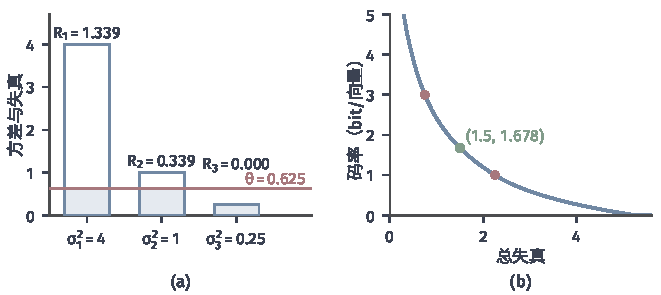
\includegraphics[width=112mm]{figures/07-probability/05-source-coding/matplotlib/rd-reverse-waterfilling/figure.pdf}
  \caption{方差为$(4,1,0.25)$的独立高斯分量的反注水。(a)总失真$1.5$时的分配：蓝框是各分量方差，浅蓝填充是分到的失真$D_k=\min\{\theta,\sigma_k^{2}\}$，红线是水平$\theta=0.625$，柱上方是各分量的码率（bit）。(b)每向量的总码率随总失真的变化；红点是分量开始或停止被描述的折点$D=0.75$与$D=2.25$，绿点是(a)中的分配。}
  \label{fig:rd-reverse-waterfilling}
\end{BookInlineFigure}

\paragraph{相关的高斯向量}
分量相关时先旋转坐标。设$\bm{X}\sim\mathcal{N}(\bm{0},\bm{\Sigma})$，协方差矩阵$\bm{\Sigma}$有正交特征分解$\bm{\Sigma}=\bm{U}\bm{\Lambda}\bm{U}^{\top}$，$\bm{\Lambda}$为特征值$\lambda_1,\dots,\lambda_m$组成的对角矩阵。令$\bm{Y}=\bm{U}^{\top}\bm{X}$，则$\bm{Y}\sim\mathcal{N}(\bm{0},\bm{\Lambda})$，各分量不相关。由第~\ref{chap:multivariate-distributions}章，联合高斯向量的分量不相关即独立。

旋转不改变问题。对任意重构$\hat{\bm{X}}$，令$\hat{\bm{Y}}=\bm{U}^{\top}\hat{\bm{X}}$。正交矩阵保持长度，
\[
  \lVert\bm{X}-\hat{\bm{X}}\rVert_2^{2}=\lVert\bm{Y}-\hat{\bm{Y}}\rVert_2^{2};
\]
$\bm{U}^{\top}$是可逆的连续映射，由第~\ref{chap:information-measures}章，双方向可测的一一变换保持互信息，$I(\bm{X};\hat{\bm{X}})=I(\bm{Y};\hat{\bm{Y}})$。所以两个问题的可行集合一一对应，目标值相同，$\bm{X}$的$R(D)$就是对特征值$\lambda_k$作反注水。

例如$\bm{\Sigma}=\begin{bmatrix}2&1\\1&2\end{bmatrix}$，特征值为$3$与$1$，特征向量为$(1,1)/\sqrt2$与$(-1,1)/\sqrt2$。总失真$D=1$时，试$\theta<1$，得$2\theta=1$，$\theta=0.5$，
\[
  R(1)=\frac12\log_2\frac{3}{0.5}+\frac12\log_2\frac{1}{0.5}\approx1.292+0.5=1.792
\]
bit每向量。若忽略相关性，把$X_1,X_2$当作两个方差为$2$的信源分别描述，最好的分法是各给$0.5$，需要$\frac12\log_2\frac{2}{0.5}\times2=2$\,bit。联合描述省下约$0.21$\,bit，来源于旋转后两个方向的方差不再相等，反注水可以把预算向方差大的方向倾斜。

\begin{BookInlineFigure}
  \centering
  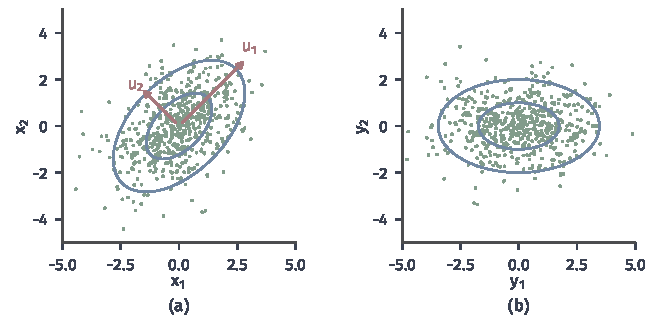
\includegraphics[width=112mm]{figures/07-probability/05-source-coding/matplotlib/rd-correlated-rotation/figure.pdf}
  \caption{相关高斯向量的旋转，$\bm{\Sigma}=\begin{bmatrix}2&1\\1&2\end{bmatrix}$，$600$个样本（绿），随机种子$722$。(a)原坐标中的样本与一倍、两倍标准差的等密度椭圆（蓝），红箭头是特征方向$\bm{u}_1,\bm{u}_2$。(b)旋转后$\bm{Y}=\bm{U}^{\top}\bm{X}$的样本，两个坐标不相关，方差分别为$3$与$1$。}
  \label{fig:rd-correlated-rotation}
\end{BookInlineFigure}

图~\ref{fig:rd-correlated-rotation}显示了旋转的作用：原坐标中两个分量一起变化，旋转后椭圆的轴与坐标轴对齐。旋转本身不改变失真和信息，它只是把问题变成可以逐分量求解的形式；码率的分配仍由特征值与水平$\theta$决定。


\section{率失真函数的计算}
\label{sec:rd-computation}

一般的有限概率表没有闭式解。第~\ref{sec:rd-feasible-range}节的三元例子只在$D_{\min}$一点能手算，整条曲线就需要数值方法。式~\eqref{eq:rd-information-rd}是一个凸优化问题，但目标中的$r_q$又依赖$q$，直接求解并不方便。Blahut–Arimoto算法把它拆成两个都有闭式解的子问题，交替求解。本节设$\mathcal{X},\hat{\mathcal{X}}$有限，$p(x)>0$对一切$x$成立（概率为零的源值可以删去），失真矩阵$d(x,\hat{x})$取非负有限值。

\paragraph{用乘子去掉约束}
失真约束先换成罚项。对$s\geq0$，令
\begin{equation}
  F_s^{\star}=\min_{q}\Bigl[I(P_X,q)+s\,\mathbb{E}d(X,\hat{X})\Bigr],
  \label{eq:rd-lagrangian}
\end{equation}
$s$称为失真乘子，单位是bit每单位失真。最小值存在，因为目标在测试信道的紧集上连续。

设$q_s$是一个最小点，$D_s$是它的平均失真。若有平均失真不超过$D_s$而互信息更小的测试信道，它的目标值也更小，与$q_s$最小矛盾。所以$I(P_X,q_s)=R(D_s)$，最小点总落在率失真曲线上。

在码率—失真平面上，目标值为常数$F$的点组成斜率为$-s$的直线$R=F-sD$。求最小就是把这条直线从下方向上平移，直到碰到可行点，第一次碰到的位置就是曲线上斜率为$-s$的切点。图~\ref{fig:rd-ba-curves}(b)画出了三条这样的支撑直线。改变$s$，切点沿曲线移动：$s$大表示失真贵，切点靠近$D_{\min}$；$s$小表示码率贵，切点靠近$D_{\max}$。

\paragraph{两个变量的目标}
困难在于$I(P_X,q)$的分母$r_q$也随$q$变化。把它换成一个自由变量。对$\hat{\mathcal{X}}$上的任一分布$r$（在$r_q>0$处$r>0$），按$\hat{x}$合并后可得
\[
  \sum_{x,\hat{x}}p(x)q(\hat{x}\mid x)\log_2\frac{q(\hat{x}\mid x)}{r(\hat{x})}
  =I(P_X,q)+\sum_{\hat{x}}r_q(\hat{x})\log_2\frac{r_q(\hat{x})}{r(\hat{x})},
\]
最后一项是$D_{\mathrm{KL}}(r_q\Vert r)\geq0$，$r=r_q$时为零。所以互信息是左端对$r$的最小值。

于是令
\begin{equation}
  J(q,r)=\sum_{x}p(x)\sum_{\hat{x}}q(\hat{x}\mid x)\Bigl[\log_2\frac{q(\hat{x}\mid x)}{r(\hat{x})}+s\,d(x,\hat{x})\Bigr],
  \label{eq:rd-ba-objective}
\end{equation}
则$F_s^{\star}=\min_{q,r}J(q,r)$。对两个变量交替求最小，每一步都有闭式解。

\paragraph{固定$r$求$q$}
引入
\begin{equation}
  Z_r(x)=\sum_{\hat{x}}r(\hat{x})\,2^{-s\,d(x,\hat{x})},\qquad
  w_r(\hat{x}\mid x)=\frac{r(\hat{x})\,2^{-s\,d(x,\hat{x})}}{Z_r(x)}.
  \label{eq:rd-ba-q-update}
\end{equation}
$w_r(\cdot\mid x)$是一个概率分布：把当前的重构边缘乘以失真的指数权重$2^{-sd}$，再归一化。由$s\,d=-\log_2(2^{-sd})$，式~\eqref{eq:rd-ba-objective}方括号中的量可以写成
\[
  \log_2\frac{q(\hat{x}\mid x)}{r(\hat{x})2^{-s\,d(x,\hat{x})}}=\log_2\frac{q(\hat{x}\mid x)}{w_r(\hat{x}\mid x)}-\log_2Z_r(x).
\]
代回去，得到
\[
  J(q,r)=\sum_{x}p(x)\,D_{\mathrm{KL}}\bigl(q(\cdot\mid x)\Vert w_r(\cdot\mid x)\bigr)-\sum_{x}p(x)\log_2Z_r(x).
\]
KL散度非负且只在两分布相同时为零，所以固定$r$时最优的$q$恰是$w_r$，最小值为
\begin{equation}
  J(w_r,r)=-\sum_{x}p(x)\log_2Z_r(x).
  \label{eq:rd-ba-j-value}
\end{equation}

式~\eqref{eq:rd-ba-q-update}有直观的含义：给定$x$，一个重构值被选中的机会正比于两件事的乘积，一是它在当前方案中被用到的频率$r(\hat{x})$，二是它离$x$有多近。失真每增加$1$，权重就乘以$2^{-s}$。

\paragraph{固定$q$求$r$}
由前面的分解，固定$q$时最优的$r$就是$r_q$，即式~\eqref{eq:rd-output-marginal}。把两步合起来，新的重构边缘是
\begin{equation}
  r^{\mathrm{new}}(\hat{x})=\sum_{x}p(x)\,w_r(\hat{x}\mid x)=r(\hat{x})\,c_r(\hat{x}),\qquad
  c_r(\hat{x})=\sum_{x}\frac{p(x)\,2^{-s\,d(x,\hat{x})}}{Z_r(x)} .
  \label{eq:rd-ba-r-update}
\end{equation}
$c_r(\hat{x})$是一个乘性修正因子：大于$1$的重构值在新方案中被用得更多。由$Z_r$的定义，
\[
  \sum_{\hat{x}}r(\hat{x})c_r(\hat{x})=\sum_{x}\frac{p(x)}{Z_r(x)}\sum_{\hat{x}}r(\hat{x})2^{-s\,d(x,\hat{x})}=\sum_xp(x)=1,
\]
所以$r^{\mathrm{new}}$仍是概率分布，且$\max_{\hat{x}}c_r(\hat{x})\geq1$。若某个$r(\hat{x})=0$，它以后永远为零，因此初值必须处处为正。

\paragraph{计算过程}
下面结合同一个例子写出计算过程。仍取$X\sim\operatorname{Bern}(0.3)$与Hamming失真，乘子取$s=\log_29\approx3.170$，于是一次错误的权重是$2^{-s}=\tfrac19$。由第~\ref{sec:rd-binary}节，$R'(D)=-\log_2\frac{1-D}{D}$，斜率为$-\log_29$的点是$D=0.1$，所以算法应收敛到$R(0.1)\approx0.4123$，目标最优值为
\[
  F_s^{\star}=R(0.1)+0.1\log_29\approx0.4123+0.3170=0.7293 .
\]

\needspace{6\baselineskip}
\paragraph{变量}
\begin{itemize}
  \item $\bm{A}$：$\lvert\mathcal{X}\rvert\times\lvert\hat{\mathcal{X}}\rvert$矩阵，元素$a_{x,\hat{x}}=2^{-s\,d(x,\hat{x})}$，计算一次后不变。例中$\bm{A}=\begin{bmatrix}1&1/9\\1/9&1\end{bmatrix}$。
  \item $r$：长度$\lvert\hat{\mathcal{X}}\rvert$的概率向量，当前重构边缘$r^{(t)}$。
  \item $Z$：长度$\lvert\mathcal{X}\rvert$的向量，归一化常数$Z^{(t)}(x)$。
  \item $q$：$\lvert\mathcal{X}\rvert\times\lvert\hat{\mathcal{X}}\rvert$矩阵，本轮的测试信道$q^{(t+1)}$，每行和为$1$。
  \item $c$：长度$\lvert\hat{\mathcal{X}}\rvert$的修正因子。
  \item $J^{(t+1)}$与$\epsilon^{(t+1)}$：本轮目标值与最优性误差界，用于停止判断；$D^{(t+1)}$与$I^{(t+1)}$：本轮测试信道的平均失真与互信息，用于报告结果。
\end{itemize}

\paragraph{初始化}
$r^{(0)}$取处处为正的分布，常用均匀分布；给定停止容差$\varepsilon>0$与最大轮数。例中
\[
  r^{(0)}=(0.5,\,0.5),\qquad \varepsilon=10^{-3}.
\]

\needspace{6\baselineskip}
\paragraph{每轮更新}
第$t+1$轮（$t=0,1,\dots$）：
\begin{enumerate}
  \item \textbf{归一化常数。}按式~\eqref{eq:rd-ba-q-update}，取$r=r^{(t)}$算出$Z^{(t)}(x)$，即矩阵$\bm{A}$的第$x$行与$r^{(t)}$的内积。例中第一轮
  \[
    Z^{(0)}(0)=0.5+\frac{0.5}{9}=\frac59,\qquad Z^{(0)}(1)=\frac{0.5}{9}+0.5=\frac59 .
  \]

  \item \textbf{测试信道。}按式~\eqref{eq:rd-ba-q-update}，$q^{(t+1)}$的第$x$行是$r^{(t)}$与$\bm{A}$第$x$行的逐元素乘积除以$Z^{(t)}(x)$。例中第一轮
  \[
    \begin{gathered}
    q^{(1)}(0\mid0)=\frac{0.5}{5/9}=0.9,\qquad q^{(1)}(1\mid0)=0.1,\\
    q^{(1)}(1\mid1)=0.9,\qquad q^{(1)}(0\mid1)=0.1 ,
    \end{gathered}
  \]
  正是第~\ref{sec:rd-test-channels}节以$0.1$翻转的测试信道。

  \item \textbf{目标值。}由式~\eqref{eq:rd-ba-j-value}，$J^{(t+1)}=-\sum_xp(x)\log_2Z^{(t)}(x)$。例中第一轮
  \[
    J^{(1)}=-\log_2\frac59\approx0.8480 .
  \]

  \item \textbf{修正因子与新边缘。}按式~\eqref{eq:rd-ba-r-update}算$c$与$r^{(t+1)}=r^{(t)}c$。例中第一轮
  \[
    c(0)=\frac{0.7\times1+0.3\times\frac19}{5/9}=1.32,\qquad c(1)=\frac{0.7\times\frac19+0.3\times1}{5/9}=0.68,
  \]
  \[
    r^{(1)}=(0.5\times1.32,\ 0.5\times0.68)=(0.66,\ 0.34).
  \]

  \item \textbf{误差界与停止。}令$\epsilon^{(t+1)}=\max_{\hat{x}}\log_2c(\hat{x})$。下面的定理~\ref{thm:rd-ba-bounds}说明最优值被夹在$J^{(t+1)}-\epsilon^{(t+1)}$与$J^{(t+1)}$之间。若$\epsilon^{(t+1)}\leq\varepsilon$则停止，否则进入下一轮。例中第一轮
  \[
    \epsilon^{(1)}=\log_21.32\approx0.4005,
  \]
  所以$F_s^{\star}\in[0.4475,\,0.8480]$，继续。

  \item \textbf{报告量。}按式~\eqref{eq:rd-test-distortion}与式~\eqref{eq:rd-test-information}算$q^{(t+1)}$的平均失真$D^{(t+1)}$与互信息$I^{(t+1)}$。例中第一轮
  \[
    D^{(1)}=0.1,\qquad I^{(1)}\approx0.4558 .
  \]
\end{enumerate}

第二轮从$r^{(1)}=(0.66,0.34)$出发：
\[
  Z^{(1)}(0)=0.66+\frac{0.34}{9}\approx0.6978,\qquad Z^{(1)}(1)=\frac{0.66}{9}+0.34\approx0.4133 .
\]
测试信道变为$q^{(2)}(1\mid0)\approx0.0541$，$q^{(2)}(0\mid1)\approx0.1774$，错误开始向罕见符号转移。目标值与修正因子为
\[
  J^{(2)}\approx0.7458,\qquad c\approx(1.0838,\ 0.8373),\qquad r^{(2)}\approx(0.7153,\ 0.2847),
\]
误差界$\epsilon^{(2)}\approx0.1161$，报告量$D^{(2)}\approx0.0911$，$I^{(2)}\approx0.4468$。

此后各轮的结果列在表~\ref{tab:rd-ba-rounds}中。误差界每轮约缩小为原来的$0.4$倍，第$7$轮的误差界约为$1.2\times10^{-3}$，第$8$轮约为$5.1\times10^{-4}$，首次低于$\varepsilon$，停止。最终得到
\[
  \begin{gathered}
  q^{(8)}(1\mid0)\approx0.0358,\qquad q^{(8)}(0\mid1)\approx0.2495,\\
  D^{(8)}\approx0.0999,\qquad I^{(8)}\approx0.4125 ,
  \end{gathered}
\]
与精确解$q(1\mid0)=\tfrac1{28}\approx0.0357$、$q(0\mid1)=0.25$、$(D,R)=(0.1,0.4123)$相差不到$10^{-3}$。

\begin{BookInlineTable}
  \centering
  \caption{Blahut–Arimoto算法在例中的各轮结果，$s=\log_29$，$r^{(0)}=(0.5,0.5)$。$r^{(t)}(1)$是本轮更新后的重构边缘，其余各量由本轮开始时的边缘$r^{(t-1)}$算出。}
  \label{tab:rd-ba-rounds}
  \begin{tabular}{cccccc}
    \toprule
    $t$ & $r^{(t)}(1)$ & $J^{(t)}$ & $\epsilon^{(t)}$ & $D^{(t)}$ & $I^{(t)}$ \\
    \midrule
    $1$ & $0.3400$ & $0.8480$ & $0.4005$ & $0.1000$ & $0.4558$ \\
    $2$ & $0.2847$ & $0.7458$ & $0.1161$ & $0.0911$ & $0.4468$ \\
    $3$ & $0.2642$ & $0.7318$ & $0.0408$ & $0.0951$ & $0.4288$ \\
    $4$ & $0.2559$ & $0.7297$ & $0.0160$ & $0.0978$ & $0.4196$ \\
    $5$ & $0.2525$ & $0.7294$ & $0.0066$ & $0.0990$ & $0.4155$ \\
    $6$ & $0.2511$ & $0.7293$ & $0.0028$ & $0.0996$ & $0.4137$ \\
    $7$ & $0.2505$ & $0.7293$ & $0.0012$ & $0.0998$ & $0.4129$ \\
    $8$ & $0.2502$ & $0.7293$ & $0.0005$ & $0.0999$ & $0.4125$ \\
    \bottomrule
  \end{tabular}
\end{BookInlineTable}

\paragraph{误差界}
停止条件依赖一个可计算的最优性误差界。它来自对任意测试信道成立的一个下界。

\begin{theorem}[Blahut–Arimoto的上下界]
\label{thm:rd-ba-bounds}
对任一处处为正的分布$r$，记$Z_r,w_r,c_r$如式~\eqref{eq:rd-ba-q-update}与式~\eqref{eq:rd-ba-r-update}。则对任意测试信道$q$，
\begin{equation}
  I(P_X,q)+s\,\mathbb{E}_qd\geq-\sum_{x}p(x)\log_2Z_r(x)-\sum_{\hat{x}}r_q(\hat{x})\log_2c_r(\hat{x}),
  \label{eq:rd-ba-lower}
\end{equation}
因而
\begin{equation}
  -\sum_xp(x)\log_2Z_r(x)-\max_{\hat{x}}\log_2c_r(\hat{x})\leq F_s^{\star}\leq-\sum_xp(x)\log_2Z_r(x).
  \label{eq:rd-ba-bounds}
\end{equation}
\end{theorem}

\begin{proof}
由$J$的分解，取$r=r_q$时$J(q,r_q)=I(P_X,q)+s\,\mathbb{E}_qd$。下面用$w_r$改写$J(q,r_q)$。由$w_r$的定义，$2^{s\,d}=r/(w_rZ_r)$，于是
\[
  \log_2\frac{q(\hat{x}\mid x)\,2^{s\,d(x,\hat{x})}}{r_q(\hat{x})}
  =\log_2\frac{q(\hat{x}\mid x)}{w_r(\hat{x}\mid x)}+\log_2\frac{r(\hat{x})}{r_q(\hat{x})}-\log_2Z_r(x).
\]
按$p(x)q(\hat{x}\mid x)$求和，左端是$I(P_X,q)+s\,\mathbb{E}_qd$，右端第三项给出$-\sum_xp(x)\log_2Z_r(x)$，第二项给出$-D_{\mathrm{KL}}(r_q\Vert r)$。

第一项对每个$\hat{x}$用引理~\ref{lem:rd-log-sum}，以$a_x=p(x)q(\hat{x}\mid x)$、$b_x=p(x)w_r(\hat{x}\mid x)$合并$x$：
\[
  \sum_{x,\hat{x}}p(x)q(\hat{x}\mid x)\log_2\frac{q(\hat{x}\mid x)}{w_r(\hat{x}\mid x)}
  \geq\sum_{\hat{x}}r_q(\hat{x})\log_2\frac{r_q(\hat{x})}{r(\hat{x})c_r(\hat{x})},
\]
这里用了式~\eqref{eq:rd-ba-r-update}：$w_r$的输出边缘是$rc_r$。右端等于$D_{\mathrm{KL}}(r_q\Vert r)-\sum_{\hat{x}}r_q(\hat{x})\log_2c_r(\hat{x})$。

三项相加，$D_{\mathrm{KL}}(r_q\Vert r)$恰好抵消，得到式~\eqref{eq:rd-ba-lower}。右端最后一项不超过$\max_{\hat{x}}\log_2c_r(\hat{x})$，对$q$取最小即得式~\eqref{eq:rd-ba-bounds}的左半。右半来自$w_r$本身的目标值：它不小于$F_s^{\star}$，又不超过$J(w_r,r)$，而后者由式~\eqref{eq:rd-ba-j-value}给出。
\end{proof}

误差界$\max_{\hat{x}}\log_2c_r(\hat{x})$为零，当且仅当所有$c_r(\hat{x})\leq1$；由$\sum_{\hat{x}}rc_r=1$，这时在$r>0$处$c_r=1$，$r$是更新的不动点。所以$\epsilon$同时度量“离不动点多远”与“离最优值多远”。

\paragraph{收敛}
误差界说明了何时可以停止，但没有说明它一定会变小。下面的定理给出目标值的收敛速度。

\begin{theorem}[目标值的收敛]
\label{thm:rd-ba-convergence}
设初值$r^{(0)}$处处为正，按上面的两步交替迭代，$J^{(t)}$是由$r^{(t-1)}$按式~\eqref{eq:rd-ba-j-value}算出的目标值。设$q^{\star}$是式~\eqref{eq:rd-lagrangian}的一个最小点，$r^{\star}=r_{q^{\star}}$。则$J^{(t)}$非增，并且
\begin{equation}
  J^{(T)}-F_s^{\star}\leq\frac{D_{\mathrm{KL}}(r^{\star}\Vert r^{(0)})}{T},\qquad T=1,2,\dots .
  \label{eq:rd-ba-rate}
\end{equation}
\end{theorem}

\begin{proof}
\emph{单调。}$J^{(t+1)}$是$J(\cdot,r^{(t)})$的最小值，$r^{(t)}$又是$J(q^{(t)},\cdot)$的最小点，所以
\[
  J^{(t+1)}=\min_qJ(q,r^{(t)})\leq J(q^{(t)},r^{(t)})\leq J(q^{(t)},r^{(t-1)})=J^{(t)}.
\]

\emph{每轮的进展。}在式~\eqref{eq:rd-ba-lower}中取$q=q^{\star}$与$r=r^{(t)}$，左端是$F_s^{\star}$，于是
\[
  J^{(t+1)}-F_s^{\star}\leq\sum_{\hat{x}}r^{\star}(\hat{x})\log_2c_{r^{(t)}}(\hat{x}).
\]
由式~\eqref{eq:rd-ba-r-update}，$c_{r^{(t)}}=r^{(t+1)}/r^{(t)}$。初值处处为正，而$2^{-sd}>0$使每个$c$为正，所以各$r^{(t)}$处处为正，右端可以写成
\[
  \sum_{\hat{x}}r^{\star}(\hat{x})\log_2\frac{r^{(t+1)}(\hat{x})}{r^{(t)}(\hat{x})}
  =D_{\mathrm{KL}}(r^{\star}\Vert r^{(t)})-D_{\mathrm{KL}}(r^{\star}\Vert r^{(t+1)}).
\]

\emph{求和。}对$t=0,\dots,T-1$相加，右端逐项相消，
\[
  \sum_{t=1}^{T}\bigl(J^{(t)}-F_s^{\star}\bigr)\leq D_{\mathrm{KL}}(r^{\star}\Vert r^{(0)})-D_{\mathrm{KL}}(r^{\star}\Vert r^{(T)})\leq D_{\mathrm{KL}}(r^{\star}\Vert r^{(0)}).
\]
由单调性，左端每一项都不小于$J^{(T)}-F_s^{\star}$，于是得到式~\eqref{eq:rd-ba-rate}。
\end{proof}

初值处处为正保证$D_{\mathrm{KL}}(r^{\star}\Vert r^{(0)})$有限；若某个最优重构值的初始概率为零，它永远回不来，算法可能停在非最优点。由$F_s^{\star}\leq I^{(t)}+sD^{(t)}\leq J^{(t)}$，所报告测试信道的目标值也以同样的速度逼近最优值；再由测试信道集合的紧性与目标的连续性，$q^{(t)}$的每个极限点都是最小点。

例中$r^{\star}=(0.75,0.25)$，
\[
  D_{\mathrm{KL}}(r^{\star}\Vert r^{(0)})=0.75\log_21.5+0.25\log_20.5\approx0.1887 .
\]
式~\eqref{eq:rd-ba-rate}保证第$8$轮的误差不超过$0.024$，实际误差只有约$4\times10^{-7}$。图~\ref{fig:rd-ba-iterations}显示，这个例子中误差按几何速度下降，比$1/T$快得多；$1/T$是对一切有限概率表都成立的保证，几何速度则依赖具体问题。

\begin{BookInlineFigure}
  \centering
  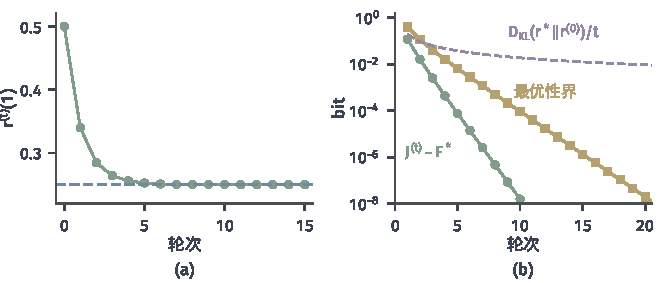
\includegraphics[width=112mm]{figures/07-probability/05-source-coding/matplotlib/rd-ba-iterations/figure.pdf}
  \caption{Blahut–Arimoto算法在例中的收敛，$s=\log_29$，$r^{(0)}=(0.5,0.5)$。(a)重构边缘$r^{(t)}(1)$（绿），蓝色虚线是极限$0.25$。(b)对数刻度下的目标误差$J^{(t)}-F_s^{\star}$（绿）、可计算的误差界$\epsilon^{(t)}=\max\log_2c$（黄）与定理~\ref{thm:rd-ba-convergence}的保证$D_{\mathrm{KL}}(r^{\star}\Vert r^{(0)})/t$（紫色虚线）。}
  \label{fig:rd-ba-iterations}
\end{BookInlineFigure}

\paragraph{改变乘子描出曲线}
每个$s$只给出曲线上的一个点$(D^{(t)},I^{(t)})$，失真不是事先指定的。要得到整条曲线，就对一列$s$分别运行；要求指定$D$处的$R(D)$，就利用$D_s$随$s$增大而不增，对$s$作二分。图~\ref{fig:rd-ba-curves}(a)对$24$个$s$运行算法，所得的点都落在式~\eqref{eq:rd-binary}的曲线上。

\begin{BookInlineFigure}
  \centering
  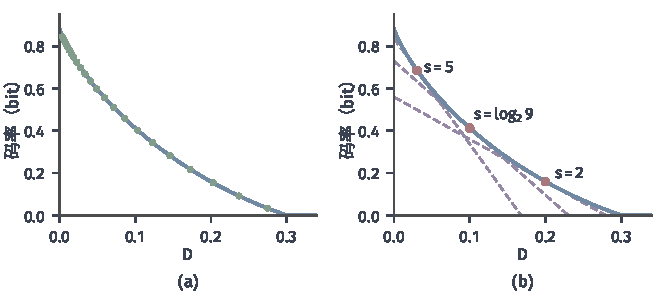
\includegraphics[width=112mm]{figures/07-probability/05-source-coding/matplotlib/rd-ba-curves/figure.pdf}
  \caption{改变乘子描出$\operatorname{Bern}(0.3)$与Hamming失真的率失真曲线。(a)$s$从$1.4$到$8$等距取$24$个值，算法的输出（绿点）落在闭式曲线$h_2(0.3)-h_2(D)$（蓝）上。(b)$s=2,\log_29,5$时目标的等值线$R=F_s^{\star}-sD$（紫色虚线）是曲线的支撑直线，红点是切点$D_s=1/(1+2^{s})$。}
  \label{fig:rd-ba-curves}
\end{BookInlineFigure}

$s$很小时，码率极贵，最优点停在零码率处。例中曲线在$D_{\max}=0.3$左侧的斜率是$-\log_2\frac{0.7}{0.3}\approx-1.222$，所以$s\leq1.222$时最小点是$(0.3,0)$；这时迭代中$r^{(t)}(1)$缓慢趋于零，收敛变慢。$s\to\infty$时切点趋于$D_{\min}$，但对有限的$s$一般到不了端点。$R(D_{\min})$可以另算：只允许把每个$x$送到使$d(x,\cdot)$最小的重构值，在这个子集上最小化互信息，这是同一类型、失真项消失的问题；第~\ref{sec:rd-feasible-range}节的三元例子就是这样算出$0.6$的。

\paragraph{线性区段}
若$R(D)$在某个区间$[D_1,D_2]$上是直线，斜率为$-s_0$，则$s=s_0$时这一段上的所有点都使式~\eqref{eq:rd-lagrangian}最小，算法收敛到哪一个取决于初值，改变$s$也只会在两个端点之间跳跃。这时先用略大和略小于$s_0$的乘子求出两个端点的测试信道，中间的点用它们的混合得到：由引理~\ref{lem:rd-mi-convex}，混合信道的互信息不超过弦的高度，而在线性区段上弦就是曲线本身。在块编码中，这对应于两种码的分时。反过来，曲线在某点有折角时，一段$s$都对应同一个点，二分得到的$D_s$会在这里停留。

\paragraph{计算代价}
每轮要算$Z$、$q$、$c$，各需$O(\lvert\mathcal{X}\rvert\lvert\hat{\mathcal{X}}\rvert)$次运算，存储$\bm{A}$与$q$需要同样大小的空间。数值上，$s$很大时$2^{-sd}$可能下溢，常把每行的指数减去该行的最小失真再计算，归一化后结果不变。还需注意算法求出的是信息率失真函数及其测试信道。它告诉我们极限是多少，以及随机码本应按什么边缘生成，但不给出有限块长的编码器。


\section{本章小结}
\label{sec:rd-summary}

本章回答了开头的两个问题。下雨概率为$0.3$的记录，允许错$10\%$时每天只需$R(0.1)=h_2(0.3)-h_2(0.1)\approx0.412$\,bit，不到无损所需的一半。标准高斯测量值每个$1$\,bit时，长块编码的均方误差极限是$0.25$，逐个量化的最好结果是$0.363$。两处都是“允许失真的最低渐近码率”与“有限方案实际做到的”之间的比较。

这个比较涉及三个层次的对象，它们回答不同的问题，使用的标准必须相同：同一个源分布、同一个失真函数、期望失真、以每个源符号的bit数计的码率。
\begin{itemize}
  \item 有限方案，如第~\ref{chap:quantization}章的量化器或第~\ref{sec:rd-block-model}节的小块长码，可以直接执行，性能可以精确计算，但只是可达区域中的一个点。
  \item 信息率失真函数$R(D)$是单个符号上的凸优化：在平均失真不超过$D$的测试信道中最小化互信息。它非增、凸，在$[D_{\min},D_{\max}]$上严格递减，可以解析或数值地求出。
  \item 操作率失真函数$R_{\mathrm{op}}(D)$是所有块长、所有码本的极限。编码定理说明，对有限字母表、无记忆信源与有界可分失真，它与$R(D)$相等。
\end{itemize}

编码定理的两半依赖不同的工具。下界从“编号只有$M$个值”出发，经数据处理、独立性与链式法则拆成单个符号，再用互信息对测试信道的凸性合并；无记忆性与可分失真在其中缺一不可。可达性用随机码本：按最优测试信道的重构边缘撒点，大数律使信息密度集中在$R(D)$附近，码字数略多于$2^{nR(D)}$就能以高概率覆盖源块，再由平均推出好码本存在。

\begin{BookInlineTable}
  \centering
  \caption{贯穿例子中几类方案的比较。上半部分为$\operatorname{Bern}(0.3)$信源与Hamming失真，下半部分为标准高斯信源与平方失真。}
  \label{tab:rd-summary}
  \begin{tabular}{lcc}
    \toprule
    方案 & 码率（bit/符号） & 平均失真 \\
    \midrule
    逐位照传 & $1$ & $0$ \\
    块长$3$，码本$\{000,100,010,001\}$ & $0.667$ & $0.081$ \\
    块长$4$，最优$4$码字码本 & $0.5$ & $0.136$ \\
    率失真极限$R(D)$ & $0.412$ & $0.1$ \\
    率失真极限$D(R)$ & $0.5$ & $0.074$ \\
    \midrule
    两点Lloyd–Max量化器 & $1$ & $0.363$ \\
    均匀量化加索引熵编码（步长$1$） & $2.105$ & $0.077$ \\
    率失真极限$D(R)=2^{-2R}$ & $1$ & $0.25$ \\
    \bottomrule
  \end{tabular}
\end{BookInlineTable}

解析解都来自同一个两步法：一个对所有测试信道成立的信息下界，加一个达到它的反向测试信道。二元信源的下界来自错误指示的熵，高斯信源的下界来自条件高斯参考与KL非负，后者与固定方差的熵上界是同一个论证。独立高斯分量的码率按反注水分配，方差低于水平的分量不描述；相关分量先按协方差的特征方向旋转，再对特征值反注水。

有限概率表用Blahut–Arimoto算法计算。乘子$s$把失真约束变成罚项，最小点是曲线上斜率为$-s$的切点；交替地用“当前边缘乘以失真的指数权重再归一化”更新测试信道、用输出边缘更新$r$，目标单调下降，误差界$\max\log_2c$可以随时计算，目标误差至少按$1/T$缩小。

求出$R(D)$还没有给出编码器。它给出的是标准：一个有限方案离极限还有多远，例如高分辨率下均匀量化加熵编码约差$0.254$\,bit，这一段只能靠联合处理多个值去缩小；以及若用随机码本，码字应按什么分布生成。有限块长的最优码与低复杂度的搜索不由本章的定理给出。

描述一个信源需要$R(D)$的码率，这些bit还要经过有噪声的信道传出去。下一部分研究信道每次使用能可靠传送多少bit，即信道容量，再把所需的描述资源与可用的传输资源放在一起比较。

